\documentclass[xcolor=dvipsnames]{beamer}

% Fonts/encoding/typography
\usepackage[utf8]{inputenc}
\usepackage{microtype}
\usepackage{csquotes}

% Links
\usepackage{hyperref}
\hypersetup{
  colorlinks=true,
  urlcolor=gray,
  linkcolor=.,
  citecolor=.
}

% Theme (fallback to default if Metropolis not installed)
\makeatletter
\@ifundefined{IfFileExists}{%
}{}
\makeatother
\IfFileExists{beamerthememetropolis.sty}{%
  \usetheme[numbering=fraction]{metropolis}
}{%
  \usetheme{default}
}

% Beamer settings
\setbeamertemplate{navigation symbols}{}
\setbeamertemplate{itemize items}[circle]
\setbeamertemplate{enumerate items}[circle]


% -------------------------------------------------------------------
% Packages
% -------------------------------------------------------------------
\usepackage{amsmath,amssymb,amsfonts}
\usepackage{mathbbol}
\usepackage{booktabs}
\usepackage{array,tabularx}
\usepackage{tikz}
\usetikzlibrary{calc,shapes.geometric}

% Compact, consistent list environments
\newenvironment{slideitems}{%
  \begin{itemize}\setlength{\itemsep}{0.55em}\setlength{\parskip}{0pt}%
}{\end{itemize}}
\newenvironment{subslideitems}{%
  \begin{itemize}\setlength{\itemsep}{0.35em}\setlength{\parskip}{0pt}%
}{\end{itemize}}
\newenvironment{slidenums}{%
  \begin{enumerate}\setlength{\itemsep}{0.55em}\setlength{\parskip}{0pt}%
}{\end{enumerate}}

% Simple quantum notation without relying on braket package syntax
\newcommand{\ket}[1]{\lvert #1\rangle}
\newcommand{\bra}[1]{\langle #1\rvert}
\newcommand{\inner}[2]{\langle #1\mid #2\rangle}
\newcommand{\C}{\mathbb{C}}
\newcommand{\myotimes}{ }

% Consistent part/section slide
\newcommand{\partslide}[2]{%
  \begin{frame}[plain]
    \centering
    \vfill
    {\Large\bfseries #1}\par\vspace{2mm}
%    {\color{Accent}\Large\bfseries #1}\par\vspace{2mm}
    {\Large\bfseries #2}
    \vfill
  \end{frame}
}

% -------------------------------------------------------------------
% Document information
% -------------------------------------------------------------------
\title{The Big Beautiful Quantum Box (BBQB):\\CSM, Quantum Logic, and Some Related Snippets}
\author{Karl Svozil\\ITP, TU Wien, Vienna, Austria}
\date{QIP26, V\"axj\"o, Sweden\\2026-06-11}

\begin{document}

% -------------------------------------------------------------------
% Title page
% -------------------------------------------------------------------
\begin{frame}[plain]
  \titlepage
\end{frame}

% ===================================================================
% PART 1 — CSM Framework vs. Quantum Logic
% ===================================================================
%\section{CSM Framework vs. Quantum Logic}
\partslide{Part I}{CSM Framework vs. Quantum Logic}

% --- SLIDE 1.1 ---
\begin{frame}[shrink=8]{CSM vs. Quantum Logic}
\footnotesize
\renewcommand{\arraystretch}{1.23}
\begin{tabularx}{\textwidth}{>{\bfseries}p{0.22\textwidth}XX}
%\toprule
 & \textbf{Quantum Logic}\newline\normalfont Birkhoff--von Neumann
 & \textbf{CSM}\newline\normalfont Contexts--Systems--Modalities \\
\midrule
Primitive notion
  & Propositions: yes/no tests, orthogonal projection operators
  & Modalities: certain, repeatable phenomena \\
Structure
  & Orthomodular lattice of projectors
  & Contexts: complete sets of $N$ mutually exclusive modalities \\
Role of context
  & Boolean subalgebras or blocks
  & Explicit and primary; a modality exists \emph{within} a context \\
Ontology
  & Properties of the system
  & Properties of system and context jointly \\
Probabilities
  & Via Gleason
  & Via Gleason/Uhlhorn \\
Goal
  & Algebraic logic of qm
  & Derive Hilbert space from desiterata \\
Common elements
  & Gleason's ``intertwining'' of observables across bases
  & Extravalence: one modality appearing in many contexts  \\
\bottomrule
\end{tabularx}

\end{frame}


% --- SLIDE 1.3 ---
\begin{frame}{Desiderata}
\begin{slideitems}
  \item In any context there are exactly $N$
        mutually exclusive modalities ($N$ fixed by the system).
  \item  The certainty of a modality can
        carry over between contexts (extravalence)---but in general
        only \emph{probabilistically}, since $N$ cannot increase.
  \item Contexts and modalities change
        continuously (connected groups of context transformations).
\end{slideitems}



\vspace{1mm}
\normalsize
\textit{Hilbert space is a formalism compatible with desiderata.}
\end{frame}

% ===================================================================
% PART 2 — Matrix Pencils, Peres–Mermin, GHZ
% ===================================================================
%\section{Matrix Pencils, Peres--Mermin Square, and GHZ Arguments}
\partslide{Part II}{Matrix Pencils, Peres--Mermin Square, and GHZ Arguments}

% --- SLIDE 2.1 ---
\begin{frame}{Matrix Pencils: Motivation}
\begin{slideitems}
  \item Operator-valued arguments can hide the underlying measurement contexts:
        orthonormal bases or projection operators.
  \item Non-degenerate operators reveal their eigensystems directly.
  \item Degenerate commuting operators require a systematic way to extract the
        common maximal-resolution context.
\end{slideitems}

\vspace{4mm}
\centering
\textit{Aim: expose the context behind a commuting family of observables.}
\end{frame}

% --- SLIDE 2.2 ---
\begin{frame}{Matrix Pencils: Construction}
Let $A_1,\dots,A_l$ be mutually commuting degenerate operators.  Form
\[
  P=\sum_{i=1}^{l} a_i A_i,
\]
where the $a_i$ are generic real scalars.

\vspace{2mm}
\begin{slideitems}
  \item $P$ commutes with every $A_i$.
  \item For generic coefficients, $P$ removes accidental degeneracies.
  \item Diagonalizing $P$ gives the simultaneous eigensystem shared by the
        commuting observables.
\end{slideitems}
\end{frame}

% --- SLIDE 2.3 ---
\begin{frame}{Peres--Mermin Square}
\begin{slideitems}
  \item The Peres--Mermin square contains nine dichotomic Pauli observables in a
        $3\times3$ grid.
  \item Each row and each column is a commuting set, giving six measurement
        contexts.
  \item Applying matrix pencils to these commuting sets reveals their common
        quantum-logical structure.
\end{slideitems}

\vspace{4mm}
\centering
\textit{The square is a compact operator form of contextuality; the pencil
extracts the underlying contexts.}
\centering
\href{https://doi.org/10.1103/PhysRevA.110.012215}{doi: 10.1103/PhysRevA.110.012215}
\end{frame}

% --- SLIDE 2.4 ---
\begin{frame}{From PM Square to KS Configurations}
\begin{slideitems}
  \item The extracted eigensystems yield a \textbf{24--24 configuration}:
        24 propositions arranged into 24 contexts.
  \item This completes the well-known \textbf{18--9 configuration} of Cabello,
        Estebaranz, and Garc\'{i}a-Alcaine.
  \item No classical two-valued truth assignment exists.
\end{slideitems}

\vspace{4mm}
\centering
\Large
\textbf{Conclusion: strong quantum contextuality.}
\end{frame}


\begin{frame}{Peres-Mermin Square}
    \begin{columns}[c]
        % Left side: Equation
        \begin{column}{0.45\textwidth}
            $
            \begin{pmatrix}
            \sigma_z \myotimes  \mathbb{1}_2 & \mathbb{1}_2 \myotimes  \sigma_z & \sigma_z \myotimes  \sigma_z \\
            \mathbb{1}_2 \myotimes  \sigma_x & \sigma_x \myotimes  \mathbb{1}_2 & \sigma_x \myotimes  \sigma_x \\
            \sigma_z \myotimes  \sigma_x & \sigma_x \myotimes  \sigma_z & \sigma_y \myotimes  \sigma_y
            \end{pmatrix}
            \qquad \equiv \qquad
            $
        \end{column}

        % Right side: TikZ Picture
        \begin{column}{0.55\textwidth}
            \centering
            \resizebox{\textwidth}{!}{%
                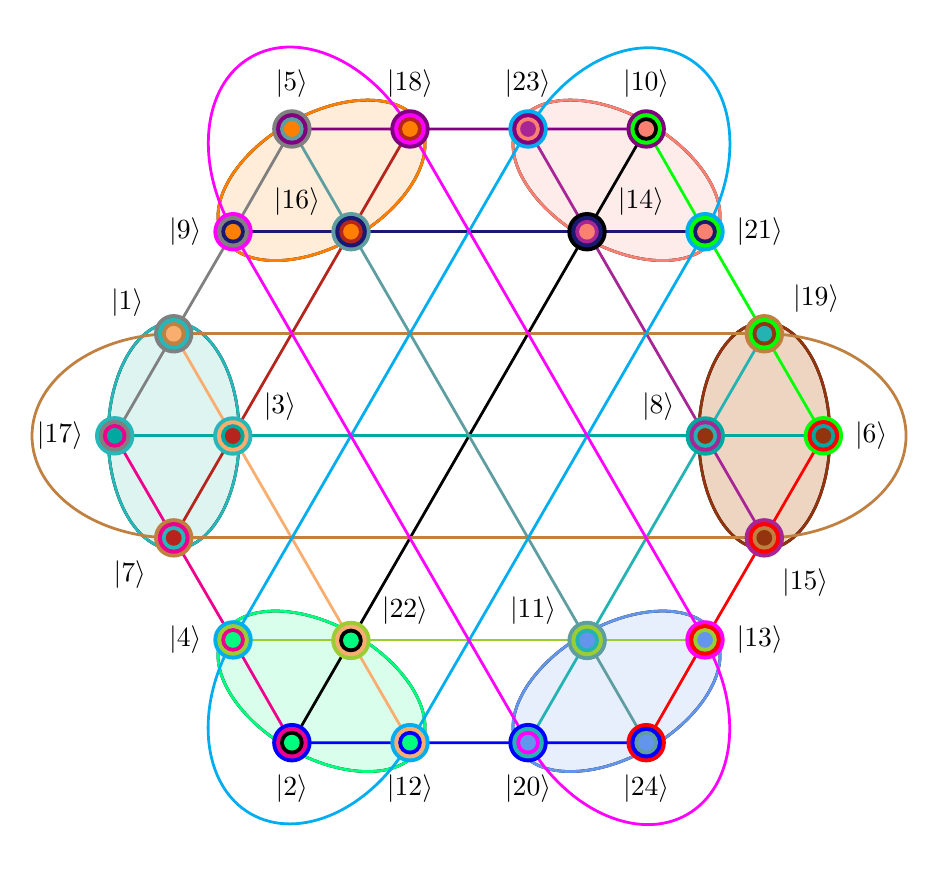
\begin{tikzpicture}[scale=0.9]
                \tikzstyle{every path}=[line width=1pt]   %,label distance=0.6pt
                \newdimen\ms
                \ms=0.1cm
                %\tikzstyle{c2}=[circle,inner sep=1pt,minimum size=5pt]
                %\tikzstyle{c1}=[circle,inner sep=0pt,minimum size=3pt]
                \tikzstyle{c4}=[circle,inner sep={\ms/8},minimum size=5*\ms]
                \tikzstyle{c3}=[circle,inner sep={\ms/8},minimum size=4*\ms]
                \tikzstyle{c2}=[circle,inner sep={\ms/8},minimum size=3*\ms]
                \tikzstyle{c1}=[circle,inner sep={\ms/8},minimum size=2*\ms]

                %%% Define positions of some observables
                \path
                      (240:5) coordinate(1)
                      (-0.833,-4.33) coordinate(2)
                      (0.833,-4.33) coordinate(3)
                      (300:5) coordinate(4)
                      (3.33,-2.88) coordinate(5)
                      (4.167,-1.44) coordinate(6)
                      (0:5) coordinate(7)
                      (4.167,1.44) coordinate(8)
                      (3.33,2.88) coordinate(9)
                      (60:5) coordinate(10)
                      (0.833,4.33) coordinate(11)
                      (-0.833,4.33) coordinate(12)
                      (120:5) coordinate(13)
                      (-3.33,2.88) coordinate(14)
                      (-4.167,1.44) coordinate(15)
                      (180:5) coordinate(16)
                      (-4.167,-1.44) coordinate(17)
                      (-3.33,-2.88) coordinate(18);

                %%% Draw all the context curves

                % small ellipses
                \node[ellipse, draw, fill=BlueGreen!15!white, minimum width=1.666cm, minimum height=2.88cm] at (-4.167,0) {};
                \node[ellipse, draw, color=BlueGreen, minimum width=1.666cm, minimum height=2.88cm] at (-4.167,0) {};
                \node[ellipse, draw, fill=RawSienna!15!white, minimum width=1.666cm, minimum height=2.88cm] at (4.167,0) {};
                \node[ellipse, draw, color=RawSienna, minimum width=1.666cm, minimum height=2.88cm] at (4.167,0) {};
                \node[ellipse, draw, fill=SpringGreen!15!white, minimum width=1.666cm, minimum height=2.88cm, rotate=60] at (-2.0815,-3.605) {};
                \node[ellipse, draw, color=SpringGreen, minimum width=1.666cm, minimum height=2.88cm, rotate=60] at (-2.0815,-3.605) {};
                \node[ellipse, draw, fill=Salmon!15!white, minimum width=1.666cm, minimum height=2.88cm, rotate=60] at ( 2.0815, 3.605) {};
                \node[ellipse, draw, color=Salmon, minimum width=1.666cm, minimum height=2.88cm, rotate=60] at ( 2.0815, 3.605) {};
                \node[ellipse, draw, fill=orange!15!white, minimum width=1.666cm, minimum height=2.88cm, rotate=-60] at (-2.0815, 3.605) {};
                \node[ellipse, draw, color=orange, minimum width=1.666cm, minimum height=2.88cm, rotate=-60] at (-2.0815, 3.605) {};
                \node[ellipse, draw, fill=CornflowerBlue!15!white, minimum width=1.666cm, minimum height=2.88cm, rotate=-60] at ( 2.0815, -3.605) {};
                \node[ellipse, draw, color=CornflowerBlue, minimum width=1.666cm, minimum height=2.88cm, rotate=-60] at ( 2.0815, -3.605) {};

                % outer hexagons
                \draw [color=green] (7) -- (8) -- (9)-- (10);
                \draw [color=violet] (10) -- (11) -- (12) -- (13);
                \draw [color=gray] (13) -- (14) -- (15) -- (16);
                \draw [color=magenta] (16) -- (17) -- (18) -- (1);
                \draw [color=blue] (1) -- (2) -- (3) -- (4);
                \draw [color=red] (4) -- (5) -- (6) -- (7);

                % inner hexagons
                \draw [color=Apricot] (2) -- (15);
                \draw [color=TealBlue] (3) -- (8);
                \draw [color=YellowGreen] (5) -- (18);
                \draw [color=MidnightBlue] (9) -- (14);
                \draw [color=Mulberry] (11) -- (6);
                \draw [color=BrickRed] (12) -- (17);

                % inner diagonals
                \draw [color=black] (1) -- (10);
                \draw [color=Emerald] (7) -- (16);
                \draw [color=CadetBlue] (4) -- (13);

                % outer ovals
                \draw [color=brown] (8) -- (15);
                \draw [color=brown](17) -- (6);
                \draw [color=brown] (8) arc (450:270:2 and 1.44);
                \draw [color=brown] (15) arc (90:270:2 and 1.44);

                \draw [color=cyan] (9) -- (2);
                \draw [color=cyan] (11) -- (18);
                \draw [rotate=240,color=cyan] (9) arc (90:270:2 and 1.44);
                \draw[rotate=60,color=cyan] (18) arc (90:270:2 and 1.44);

                \draw [color=Fuchsia] (12) -- (5);
                \draw [color=Fuchsia] (14) -- (3);
                \draw[rotate=300,color=Fuchsia] (12) arc (90:270:2 and 1.44);
                \draw[rotate=120,color=Fuchsia] (3) arc (90:270:2 and 1.44);

                % Draw the observables themselves
                \draw (1) coordinate[c4,fill=blue,label=270:$\vert 2 \rangle$];
                \draw (1) coordinate[c3,fill=magenta];
                \draw (1) coordinate[c2,fill=black];
                \draw (1) coordinate[c1,fill=SpringGreen];

                \draw (2) coordinate[c4,fill=cyan,label=270:$\vert 12 \rangle$];
                \draw (2) coordinate[c3,fill=Apricot];
                \draw (2) coordinate[c2,fill=blue];
                \draw (2) coordinate[c1,fill=SpringGreen];

                \draw (3) coordinate[c4,fill=blue,label=270:$\vert 20 \rangle$];
                \draw (3) coordinate[c3,fill=TealBlue];
                \draw (3) coordinate[c2,fill=Fuchsia];
                \draw (3) coordinate[c1,fill=CornflowerBlue];

                \draw (4) coordinate[c4,fill=red,label=270:$\vert 24 \rangle$];
                \draw (4) coordinate[c3,fill=blue];
                \draw (4) coordinate[c2,fill=CadetBlue];
                \draw (4) coordinate[c1,fill=CornflowerBlue];

                \draw (5) coordinate[c4,fill=Fuchsia,label=0:$\vert 13 \rangle$];
                \draw (5) coordinate[c3,fill=red];
                \draw (5) coordinate[c2,fill=YellowGreen];
                \draw (5) coordinate[c1,fill=CornflowerBlue];

                \draw (6) coordinate[c4,fill=Mulberry,label=290:$\vert 15 \rangle$];
                \draw (6) coordinate[c3,fill=red];
                \draw (6) coordinate[c2,fill=brown];
                \draw (6) coordinate[c1,fill=RawSienna];

                \draw (7) coordinate[c4,fill=green,label=0:$\vert 6 \rangle$];
                \draw (7) coordinate[c3,fill=red];
                \draw (7) coordinate[c2,fill=Emerald];
                \draw (7) coordinate[c1,fill=RawSienna];

                \draw (8) coordinate[c4,fill=brown,label=30:$\vert 19 \rangle$];
                \draw (8) coordinate[c3,fill=green];
                \draw (8) coordinate[c2,fill=RawSienna];
                \draw (8) coordinate[c1,fill=TealBlue];

                \draw (9) coordinate[c4,fill=cyan,label=0:$\vert 21 \rangle$];
                \draw (9) coordinate[c3,fill=green];
                \draw (9) coordinate[c2,fill=MidnightBlue];
                \draw (9) coordinate[c1,fill=Salmon];

                \draw (10) coordinate[c4,fill=violet,label=90:$\vert 10 \rangle$];
                \draw (10) coordinate[c3,fill=green];
                \draw (10) coordinate[c2,fill=black];
                \draw (10) coordinate[c1,fill=Salmon];

                \draw (11) coordinate[c4,fill=cyan,label=91:$\vert 23 \rangle$];
                \draw (11) coordinate[c3,fill=violet];
                \draw (11) coordinate[c2,fill=Salmon];
                \draw (11) coordinate[c1,fill=Mulberry];

                \draw (12) coordinate[c4,fill=violet,label=90:$\vert 18 \rangle$];
                \draw (12) coordinate[c3,fill=Fuchsia];
                \draw (12) coordinate[c2,fill=BrickRed];
                \draw (12) coordinate[c1,fill=orange];

                \draw (13) coordinate[c4,fill=gray,label=90:$\vert 5 \rangle$];
                \draw (13) coordinate[c3,fill=violet];
                \draw (13) coordinate[c2,fill=CadetBlue];
                \draw (13) coordinate[c1,fill=orange];

                \draw (14) coordinate[c4,fill=Fuchsia,label=180:$\vert 9 \rangle$];
                \draw (14) coordinate[c3,fill=gray];
                \draw (14) coordinate[c2,fill=MidnightBlue];
                \draw (14) coordinate[c1,fill=orange];

                \draw (15) coordinate[c4,fill=gray,label=160:$\vert 1 \rangle$];
                \draw (15) coordinate[c3,fill=BlueGreen];
                \draw (15) coordinate[c2,fill=brown];
                \draw (15) coordinate[c1,fill=Apricot];

                \draw (16) coordinate[c4,fill=BlueGreen,label=180:$\vert 17 \rangle$];
                \draw (16) coordinate[c3,fill=gray];
                \draw (16) coordinate[c2,fill=magenta];
                \draw (16) coordinate[c1,fill=Emerald];

                \draw (17) coordinate[c4,fill=brown,label=215:$\vert 7 \rangle$];
                \draw (17) coordinate[c3,fill=magenta];
                \draw (17) coordinate[c2,fill=BlueGreen];
                \draw (17) coordinate[c1,fill=BrickRed];

                \draw (18) coordinate[c4,fill=cyan,label=180:$\vert 4 \rangle$];
                \draw (18) coordinate[c3,fill=YellowGreen];
                \draw (18) coordinate[c2,fill=magenta];
                \draw (18) coordinate[c1,fill=SpringGreen];

                \node (19) at ($(2)!0.25!(15)$) {};  \draw (19) coordinate[c4,fill=YellowGreen,label=15:$\vert 22 \rangle$];
                \node (20) at ($(3)!0.25!(8)$) {};   \draw (20) coordinate[c4,fill=CadetBlue,label=165:$\vert 11 \rangle$];
                \node (21) at ($(3)!0.75!(8)$) {};   \draw (21) coordinate[c4,fill=Emerald,label=165:$\vert 8 \rangle$];
                \node (22) at ($(9)!0.25!(14)$) {};  \draw (22) coordinate[c4,fill=black,label=15:$\vert 14 \rangle$];
                \node (23) at ($(9)!0.75!(14)$) {};  \draw (23) coordinate[c4,fill=CadetBlue,label=165:$\vert 16 \rangle$];
                \node (24) at ($(2)!0.75!(15)$) {};  \draw (24) coordinate[c4,fill=BlueGreen,label=15:$\vert 3 \rangle$];

                \draw (19) coordinate[c3,fill=Apricot];
                \draw (19) coordinate[c2,fill=black];
                \draw (19) coordinate[c1,fill=SpringGreen];

                \draw (20) coordinate[c3,fill=YellowGreen];
                \draw (20) coordinate[c2,fill=TealBlue];
                \draw (20) coordinate[c1,fill=CornflowerBlue];

                \draw (21) coordinate[c3,fill=Mulberry];
                \draw (21) coordinate[c2,fill=TealBlue];
                \draw (21) coordinate[c1,fill=RawSienna];

                \draw (22) coordinate[c3,fill=MidnightBlue];
                \draw (22) coordinate[c2,fill=Mulberry];
                \draw (22) coordinate[c1,fill=Salmon];

                \draw (23) coordinate[c3,fill=MidnightBlue];
                \draw (23) coordinate[c2,fill=BrickRed];
                \draw (23) coordinate[c1,fill=orange];

                \draw (24) coordinate[c3,fill=Apricot];
                \draw (24) coordinate[c2,fill=Emerald];
                \draw (24) coordinate[c1,fill=BrickRed];

                \end{tikzpicture}%
            }
        \end{column}
    \end{columns}
\end{frame}

% --- SLIDE 2.5 ---
\begin{frame}{Tripartite GHZM Argument}
\begin{slideitems}
  \item Mermin's GHZM version uses four commuting three-partite operators.
  \item A matrix pencil reveals one context of eight (entangled) states.
\href{https://doi.org/10.1007/s10701-021-00515-z}{doi: 10.1007/s10701-021-00515-z} \\
  \item A parity argument gives a state-dependent contradiction.
\end{slideitems}

\centering
\Large
\textbf{Quantum prediction: $-1$}\\[1mm]
\textbf{Classical prediction: $+1$}
\end{frame}

\begin{frame}{GHZ Observables and States}

    % --- TOP SECTION ---
    \vspace{1em}
    \begin{center}
        $\sigma_x \myotimes  \sigma_x \myotimes  \sigma_x$,
        $\sigma_x \myotimes  \sigma_y \myotimes  \sigma_y$,
        $\sigma_y \myotimes  \sigma_x \myotimes  \sigma_y$, and
        $\sigma_y \myotimes  \sigma_y \myotimes  \sigma_x$.   \\
$\;$        \\
$\;$      \\

$\equiv$
    \end{center}



    % --- BOTTOM SECTION ---
    \begin{center}
        \resizebox{\textwidth}{!}{%
        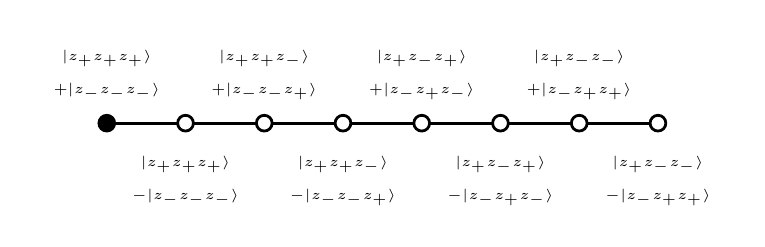
\begin{tikzpicture}[scale=1]

        \tikzstyle{every path}=[line width=1pt]

        \newdimen\ms
        \ms=0.1cm
        \tikzstyle{s1}=[color=red,rectangle,inner sep=3.5]
        \tikzstyle{c3}=[circle,inner sep={\ms/8},minimum size=4*\ms]
        \tikzstyle{c2}=[circle,inner sep={\ms/8},minimum size=3*\ms]
        \tikzstyle{c1}=[circle,inner sep={\ms/8},minimum size=2*\ms]
        \tikzstyle{cs1}=[circle,inner sep={\ms/8},minimum size=1*\ms]

        % Define positions of all observables
        \coordinate (uuu) at (0,8);
        \coordinate (uuv) at (1,8);
        \coordinate (uvu) at (2,8);
        \coordinate (uvv) at (3,8);
        \coordinate (vuu) at (4,8);
        \coordinate (vuv) at (5,8);
        \coordinate (vvu) at (6,8);
        \coordinate (vvv) at (7,8);

        % draw contexts
        \draw [color=black] (uuu) -- (vvv);

        % draw atoms
        \draw (uuu) coordinate[c1,fill=black, draw=black,label=above:{\begin{tabular}{c}\tiny $\vert z_+z_+z_+ \rangle $\\ \tiny $ + \vert z_-z_-z_- \rangle $\end{tabular}}];
        \draw (uuv) coordinate[c1,fill=white, draw=black,label=below:{\begin{tabular}{c}\tiny  $\vert z_+z_+z_+ \rangle $\\ \tiny $ - \vert z_-z_-z_- \rangle $\end{tabular}}];
        \draw (uvu) coordinate[c1,fill=white, draw=black,label=above:{\begin{tabular}{c}\tiny  $\vert z_+z_+z_- \rangle $\\ \tiny $ + \vert z_-z_-z_+ \rangle $\end{tabular}}];
        \draw (uvv) coordinate[c1,fill=white, draw=black,label=below:{\begin{tabular}{c}\tiny  $\vert z_+z_+z_- \rangle $\\ \tiny $ - \vert z_-z_-z_+ \rangle $\end{tabular}}];
        \draw (vuu) coordinate[c1,fill=white, draw=black,label=above:{\begin{tabular}{c}\tiny  $\vert z_+z_-z_+ \rangle $\\ \tiny $ + \vert z_-z_+z_- \rangle $\end{tabular}}];
        \draw (vuv) coordinate[c1,fill=white, draw=black,label=below:{\begin{tabular}{c}\tiny  $\vert z_+z_-z_+ \rangle $\\ \tiny $ - \vert z_-z_+z_- \rangle $\end{tabular}}];
        \draw (vvu) coordinate[c1,fill=white, draw=black,label=above:{\begin{tabular}{c}\tiny  $\vert z_+z_-z_- \rangle $\\ \tiny $ + \vert z_-z_+z_+ \rangle $\end{tabular}}];
        \draw (vvv) coordinate[c1,fill=white, draw=black,label=below:{\begin{tabular}{c}\tiny  $\vert z_+z_-z_- \rangle $\\ \tiny $ - \vert z_-z_+z_+ \rangle $\end{tabular}}];

        \end{tikzpicture}%
        }
    \end{center}

\end{frame}

% --- SLIDE 2.6 ---
\begin{frame}{Bipartite GHZM from the PM Square}
\begin{slideitems}
  \item A complete GHZ-type contradiction can be obtained with two particles.
  \item Use non-local observables from the last row and column of the
        Peres--Mermin square.
  \item Representative products include
        \[
          (\sigma_z\!\otimes\!\sigma_x)(\sigma_x\!\otimes\!\sigma_z),
          \qquad
          (\sigma_x\!\otimes\!\sigma_x)(\sigma_z\!\otimes\!\sigma_z).
        \]
  \item The associated matrix pencil yields the Bell basis as a single
        four-dimensional context.
\end{slideitems}
\centering
\href{https://doi.org/10.1103/PhysRevA.110.012215}{doi: 10.1103/PhysRevA.110.012215}
\end{frame}

% --- SLIDE 2.7 ---
\begin{frame}{Bipartite GHZM: Parity Contradiction}
\begin{slideitems}
  \item Classical ``elements of reality'' occur an even number of times.
  \item Therefore any classical product assignment predicts $+1$.
  \item Quantum mechanically, the product equals
$
\langle
\mathbb{1}_2 \otimes (-\mathbb{1}_2)
\rangle  =
-\langle
\mathbb{1}_4
 \rangle =
-1
 $.
\end{slideitems}

\vspace{5mm}
\centering
\Large
\textbf{Classical: $+1$}\qquad\textbf{Quantum: $-1$}
\end{frame}



\begin{frame}{The Specker bug: ``Hardy's wonderful trick'' [Mermin], also called ``Hardy's beautiful example'' [Penrose]}
\vspace{2mm}
    \begin{columns}[c]
        % --- LEFT SIDE ---
        \begin{column}{0.2\textwidth}
            \centering
            {\Large TIFS: $1 \longrightarrow 0$}
        \end{column}

        % --- RIGHT SIDE ---
        \begin{column}{0.8\textwidth}
            \centering
            \resizebox{\textwidth}{!}{%
                \begin{tabular}{ c c }

                % First TikZ Picture (a)
                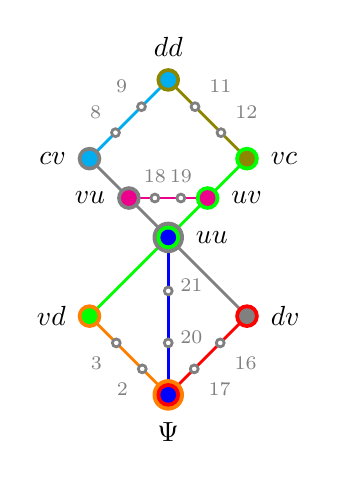
\begin{tikzpicture}[scale=0.5]
                \tikzstyle{every path}=[line width=1pt]
                \newdimen\ms
                \ms=0.1cm
                \tikzstyle{s1}=[color=red,rectangle,inner sep=3.5]
                \tikzstyle{c3}=[circle,inner sep={\ms/8},minimum size=4*\ms]
                \tikzstyle{c2}=[circle,inner sep={\ms/8},minimum size=3*\ms]
                \tikzstyle{c1}=[circle,inner sep={\ms/8},minimum size=2*\ms]
                \tikzstyle{cs1}=[circle,inner sep={\ms/8},minimum size=1*\ms]

                % Define positions of all observables
                \coordinate (psi) at (2,0);
                \coordinate (vd) at (0,2);
                \coordinate (dv) at (4,2);
                \coordinate (uu) at (2,4);
                \coordinate (vu) at (1,5);
                \coordinate (uv) at (3,5);
                \coordinate (cv) at (0,6);
                \coordinate (vc) at (4,6);
                \coordinate (dd) at (2,8);

                % draw contexts
                \draw [color=orange] (psi) -- (vd)  coordinate[cs1,fill=white,draw=gray,pos=0.33,label=below left:{\scriptsize \color{gray}2}] (2)  coordinate[cs1,fill=white,draw=gray,pos=0.66,label=below left:{\scriptsize \color{gray}3}] (3);
                \draw [color=blue] (psi) -- (uu)  coordinate[cs1,fill=white,draw=gray,pos=0.33,label={[right,xshift=0.2mm]:{\scriptsize \color{gray}20}}] (20)  coordinate[cs1,fill=white,draw=gray,pos=0.66,label={[right,xshift=0.2mm]:{\scriptsize \color{gray}21}}] (21);
                \draw [color=red] (psi) -- (dv) coordinate[cs1,fill=white,draw=gray,pos=0.33,label=below right:{\scriptsize \color{gray}17}]  (17) coordinate[cs1,fill=white,draw=gray,pos=0.66,label=below right:{\scriptsize \color{gray}16}] (16);
                \draw [color=green] (vd) -- (vc);
                \draw [color=gray] (dv) -- (cv);
                \draw [color=magenta] (vu) -- (uv) coordinate[cs1,fill=white,draw=gray,pos=0.33,label=above:{\scriptsize \color{gray}18}] (18)  coordinate[cs1,fill=white,draw=gray,pos=0.66,label=above:{\scriptsize \color{gray}19}] (19);
                \draw [color=cyan] (cv) -- (dd) coordinate[cs1,fill=white,draw=gray,pos=0.33,label=above left:{\scriptsize \color{gray}8}]  (8) coordinate[cs1,fill=white,draw=gray,pos=0.66,label=above left:{\scriptsize \color{gray}9}] (9);
                \draw [color=olive] (vc) -- (dd) coordinate[cs1,fill=white,draw=gray,pos=0.33,label=above right:{\scriptsize \color{gray}12}] (12)  coordinate[cs1,fill=white,draw=gray,pos=0.66,label=above right:{\scriptsize \color{gray}11}] (12);

                % draw atoms
                \draw (psi) coordinate[c3,fill=orange,label=below:$\Psi$];
                \draw (psi) coordinate[c2,fill=red];
                \draw (psi) coordinate[c1,fill=blue];

                \draw (vd) coordinate[c2,fill=orange,label=left:$vd$];
                \draw (vd) coordinate[c1,fill=green];

                \draw (dv) coordinate[c2,fill=red,label=right:$dv$];
                \draw (dv) coordinate[c1,fill=gray];

                \draw (uu) coordinate[c3,fill=gray,label=right:$uu$];
                \draw (uu) coordinate[c2,fill=green];
                \draw (uu) coordinate[c1,fill=blue];

                \draw (vu) coordinate[c2,fill=gray,label=left:$vu$];
                \draw (vu) coordinate[c1,fill=magenta];

                \draw (uv) coordinate[c2,fill=green,label=right:$uv$];
                \draw (uv) coordinate[c1,fill=magenta];

                \draw (cv) coordinate[c2,fill=gray,label=left:$cv$];
                \draw (cv) coordinate[c1,fill=cyan];

                \draw (vc) coordinate[c2,fill=green,label=right:$vc$];
                \draw (vc) coordinate[c1,fill=olive];

                \draw (dd) coordinate[c2,fill=olive,label=above:$dd$];
                \draw (dd) coordinate[c1,fill=cyan];
                \end{tikzpicture}

                &

                % Second TikZ Picture (b)
                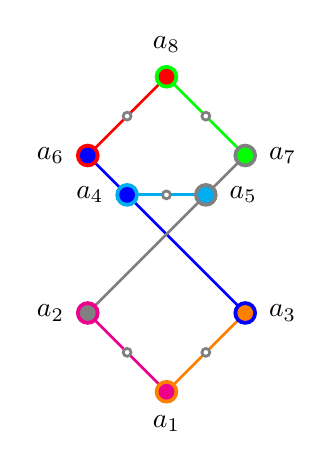
\begin{tikzpicture}[scale=1]
                \tikzstyle{every path}=[line width=1pt]
                \newdimen\ms
                \ms=0.1cm
                \tikzstyle{s1}=[color=red,rectangle,inner sep=3.5]
                \tikzstyle{c3}=[circle,inner sep={\ms/8},minimum size=5*\ms]
                \tikzstyle{c2}=[circle,inner sep={\ms/8},minimum size=3*\ms]
                \tikzstyle{c1}=[circle,inner sep={\ms/8},minimum size=2*\ms]
                \tikzstyle{cs1}=[circle,inner sep={\ms/8},minimum size=1*\ms]

                % Define positions of all observables
                \coordinate (a8) at  (1,2);
                \coordinate (a7) at (2,1);
                \coordinate (a4) at (0.5,0.5);
                \coordinate (a3) at (2,-1);
                \coordinate (a1) at (1,-2);
                \coordinate (a2) at (0,-1);
                \coordinate (a5) at (1.5,0.5);
                \coordinate (a6) at (0,1);

                % draw contexts
                \draw [color=orange] (a1) -- (a3)  coordinate[cs1,fill=white,draw=gray,pos=0.5] (2);
                \draw [color=blue] (a3) -- (a6);
                \draw [color=red] (a6) -- (a8)  coordinate[cs1,fill=white,draw=gray,pos=0.5] (7);
                \draw [color=green] (a7) -- (a8)  coordinate[cs1,fill=white,draw=gray,pos=0.5] (3);
                \draw [color=gray] (a2) -- (a7);
                \draw [color=magenta] (a2) -- (a1)  coordinate[cs1,fill=white,draw=gray,pos=0.5] (10);
                \draw [color=cyan] (a4) -- (a5)  coordinate[cs1,fill=white,draw=gray,pos=0.5] (13);

                % draw atoms
                \draw (a1) coordinate[c2,fill=orange,label=below:$a_1$];
                \draw (a1) coordinate[c1,fill=magenta];

                \draw (a2) coordinate[c2,fill=magenta,label=left:$a_{2}$];
                \draw (a2) coordinate[c1,fill=gray];

                \draw (a3) coordinate[c2,fill=blue,label=right:$a_3$];
                \draw (a3) coordinate[c1,fill=orange];

                \draw (a4) coordinate[c2,fill=cyan,label=left:$a_4$];
                \draw (a4) coordinate[c1,fill=blue];

                \draw (a5) coordinate[c2,fill=gray,label=right:$a_{5}$];
                \draw (a5) coordinate[c1,fill=cyan];

                \draw (a6) coordinate[c2,fill=red,label=left:$a_6$];
                \draw (a6) coordinate[c1,fill=blue];

                \draw (a7) coordinate[c2,fill=gray,label=right:$a_7$];
                \draw (a7) coordinate[c1,fill=green];

                \draw (a8) coordinate[c2,fill=green,label=above:$a_8$];
                \draw (a8) coordinate[c1,fill=red];
                \end{tikzpicture}
                \end{tabular}%
            }
        \end{column}
    \end{columns}

    % --- BOTTOM SECTION: REFERENCE ---


    \begingroup
    \scriptsize
    \textbf{Reference:} A. Cabello, J. M. Estebaranz, and G. Garc\'{i}a-Alcaine. \textit{Bell-Kochen-Specker theorem: A proof with 18 vectors}. Physics Letters A, 212(4): 183-187, 1996. \href{https://doi.org/10.1016/0375-9601(96)00134-X}{DOI: 10.1016/0375-9601(96)00134-X}. arXiv: \href{https://arxiv.org/abs/quant-ph/9706009}{quant-ph/9706009}.
    \endgroup

\end{frame}





\begin{frame}{Specker Bug Combo: nonseparable set of two-valued states -- strong contextuality}
    \centering
    % Shrink the entire body to fit the vertical bounds of the slide
    \resizebox*{!}{0.9\textheight}{%
    \begin{minipage}{1.6\textwidth}
        \centering

        \begin{figure}
        \centering
        \begin{tabular}{ c c c }
        \resizebox{.35\textwidth}{!}{%
        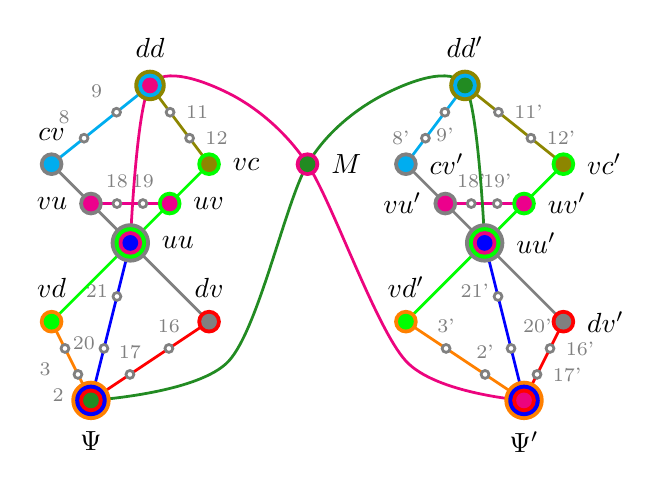
\begin{tikzpicture}  [scale=0.5]
        \tikzstyle{every path}=[line width=1pt]
        \newdimen\ms
        \ms=0.1cm
        \tikzstyle{s1}=[color=red,rectangle,inner sep=3.5]
        \tikzstyle{c4}=[circle,inner sep={\ms/8},minimum size=5*\ms]
        \tikzstyle{c3}=[circle,inner sep={\ms/8},minimum size=4*\ms]
        \tikzstyle{c2}=[circle,inner sep={\ms/8},minimum size=3*\ms]
        \tikzstyle{c1}=[circle,inner sep={\ms/8},minimum size=2*\ms]
        \tikzstyle{cs1}=[circle,inner sep={\ms/8},minimum size=1*\ms]

        \coordinate (psi) at (1,0);
        \coordinate (vd) at (0,2);
        \coordinate (dv) at (4,2);
        \coordinate (uu) at (2,4);
        \coordinate (vu) at (1,5);
        \coordinate (uv) at (3,5);
        \coordinate (cv) at (0,6);
        \coordinate (vc) at (4,6);
        \coordinate (dd) at (2.5,8);
        \coordinate (aux1) at (4.5,1);
        \coordinate (aux2) at (9,1);
        \coordinate (aux3) at (4.5,7.8);
        \coordinate (aux4) at (8.5,7.8);
        \coordinate (P) at (10.5,8);
        \coordinate (M) at (6.5,6);
        \coordinate (N) at (12,0);
        \coordinate (psi2) at ({3+9},0);
        \coordinate (vd2) at ({0+9},2);
        \coordinate (dv2) at ({4+9},2);
        \coordinate (uu2) at ({2+9},4);
        \coordinate (vu2) at ({1+9},5);
        \coordinate (uv2) at ({3+9},5);
        \coordinate (cv2) at ({0+9},6);
        \coordinate (vc2) at ({4+9},6);
        \coordinate (dd2) at ({1.5+9},8);

        \draw [color=orange] (psi) -- (vd)  coordinate[cs1,fill=white,draw=gray,pos=0.33,label=below left:{\scriptsize \color{gray}2}] (2)  coordinate[cs1,fill=white,draw=gray,pos=0.66,label=below left:{\scriptsize \color{gray}3}] (3);
        \draw [color=blue] (psi) -- (uu)  coordinate[cs1,fill=white,draw=gray,pos=0.33,label={[left,xshift=0.2mm]:{\scriptsize \color{gray}20}}] (20)  coordinate[cs1,fill=white,draw=gray,pos=0.66,label={[left,xshift=0.2mm]:{\scriptsize \color{gray}21}}] (21);
        \draw [color=red] (psi) -- (dv) coordinate[cs1,fill=white,draw=gray,pos=0.33,label=above:{\scriptsize \color{gray}17}]  (17) coordinate[cs1,fill=white,draw=gray,pos=0.66,label=above:{\scriptsize \color{gray}16}] (16);
        \draw [color=green] (vd) -- (vc);
        \draw [color=gray] (dv) -- (cv);
        \draw [color=magenta] (vu) -- (uv) coordinate[cs1,fill=white,draw=gray,pos=0.33,label=above:{\scriptsize \color{gray}18}] (18)  coordinate[cs1,fill=white,draw=gray,pos=0.66,label=above:{\scriptsize \color{gray}19}] (19);
        \draw [color=cyan] (cv) -- (dd) coordinate[cs1,fill=white,draw=gray,pos=0.33,label=above left:{\scriptsize \color{gray}8}]  (8) coordinate[cs1,fill=white,draw=gray,pos=0.66,label=above left:{\scriptsize \color{gray}9}] (9);
        \draw [color=olive] (vc) -- (dd) coordinate[cs1,fill=white,draw=gray,pos=0.33,label=right:{\scriptsize \color{gray}12}] (12)  coordinate[cs1,fill=white,draw=gray,pos=0.66,label=right:{\scriptsize \color{gray}11}] (11);
        \draw [color=orange] (psi2) -- (vd2)  coordinate[cs1,fill=white,draw=gray,pos=0.33,label=above:{\scriptsize \color{gray}2'}] (22)  coordinate[cs1,fill=white,draw=gray,pos=0.66,label=above:{\scriptsize \color{gray}3'}] (32);
        \draw [color=blue] (psi2) -- (uu2)  coordinate[cs1,fill=white,draw=gray,pos=0.33,label={[above right,xshift=0.2mm]:{\scriptsize \color{gray}20'}}] (202)  coordinate[cs1,fill=white,draw=gray,pos=0.66,label={[left,xshift=0.2mm]:{\scriptsize \color{gray}21'}}] (212);
        \draw [color=red] (psi2) -- (dv2) coordinate[cs1,fill=white,draw=gray,pos=0.33,label=right:{\scriptsize \color{gray}17'}]  (172) coordinate[cs1,fill=white,draw=gray,pos=0.66,label=right:{\scriptsize \color{gray}16'}] (162);
        \draw [color=green] (vd2) -- (vc2);
        \draw [color=gray] (dv2) -- (cv2);
        \draw [color=magenta] (vu2) -- (uv2) coordinate[cs1,fill=white,draw=gray,pos=0.33,label=above:{\scriptsize \color{gray}18'}] (182)  coordinate[cs1,fill=white,draw=gray,pos=0.66,label=above:{\scriptsize \color{gray}19'}] (192);
        \draw [color=cyan] (cv2) -- (dd2) coordinate[cs1,fill=white,draw=gray,pos=0.33,label=left:{\scriptsize \color{gray}8'}]  (82) coordinate[cs1,fill=white,draw=gray,pos=0.66,label=below:{\scriptsize \color{gray}9'}] (92);
        \draw [color=olive] (vc2) -- (dd2) coordinate[cs1,fill=white,draw=gray,pos=0.33,label=right:{\scriptsize \color{gray}12'}] (122)  coordinate[cs1,fill=white,draw=gray,pos=0.66,label=right:{\scriptsize \color{gray}11'}] (112);

        \draw [ForestGreen] plot [smooth] coordinates {(psi)  (aux1) (M) (aux4) (P) (uu2) };
        \draw [RubineRed] plot [smooth] coordinates {(uu) (dd) (aux3) (M) (aux2) (N)};

        \draw (psi) coordinate[c4,fill=orange,label=below:$\Psi$];
        \draw (psi) coordinate[c3,fill=blue];
        \draw (psi) coordinate[c2,fill=red];
        \draw (psi) coordinate[c1,fill=ForestGreen];
        \draw (vd) coordinate[c2,fill=orange,label=above:$vd$];
        \draw (vd) coordinate[c1,fill=green];
        \draw (dv) coordinate[c2,fill=red,label=above:$dv$];
        \draw (dv) coordinate[c1,fill=gray];
        \draw (uu) coordinate[c4,fill=gray,label=right:$uu$];
        \draw (uu) coordinate[c3,fill=green];
        \draw (uu) coordinate[c2,fill=RubineRed];
        \draw (uu) coordinate[c1,fill=blue];
        \draw (vu) coordinate[c2,fill=gray,label=left:$vu$];
        \draw (vu) coordinate[c1,fill=magenta];
        \draw (uv) coordinate[c2,fill=green,label=right:$uv$];
        \draw (uv) coordinate[c1,fill=magenta];
        \draw (cv) coordinate[c2,fill=gray,label=above:$cv$];
        \draw (cv) coordinate[c1,fill=cyan];
        \draw (vc) coordinate[c2,fill=green,label=right:$vc$];
        \draw (vc) coordinate[c1,fill=olive];
        \draw (dd) coordinate[c3,fill=olive,label=above:$dd$];
        \draw (dd) coordinate[c2,fill=cyan];
        \draw (dd) coordinate[c1,fill=RubineRed];
        \draw (psi2) coordinate[c4,fill=orange,label=below:$\Psi'$];
        \draw (psi2) coordinate[c3,fill=blue];
        \draw (psi2) coordinate[c2,fill=red];
        \draw (psi2) coordinate[c1,fill=RubineRed];
        \draw (vd2) coordinate[c2,fill=orange,label=above:$vd'$];
        \draw (vd2) coordinate[c1,fill=green];
        \draw (dv2) coordinate[c2,fill=red,label=right:$dv'$];
        \draw (dv2) coordinate[c1,fill=gray];
        \draw (uu2) coordinate[c4,fill=gray,label=right:$uu'$];
        \draw (uu2) coordinate[c3,fill=green];
        \draw (uu2) coordinate[c2,fill=RubineRed];
        \draw (uu2) coordinate[c1,fill=blue];
        \draw (vu2) coordinate[c2,fill=gray,label=left:$vu'$];
        \draw (vu2) coordinate[c1,fill=magenta];
        \draw (uv2) coordinate[c2,fill=green,label=right:$uv'$];
        \draw (uv2) coordinate[c1,fill=magenta];
        \draw (cv2) coordinate[c2,fill=gray,label=right:$cv'$];
        \draw (cv2) coordinate[c1,fill=cyan];
        \draw (vc2) coordinate[c2,fill=green,label=right:$vc'$];
        \draw (vc2) coordinate[c1,fill=olive];
        \draw (dd2) coordinate[c3,fill=olive,label=above:$dd'$];
        \draw (dd2) coordinate[c2,fill=cyan];
        \draw (dd2) coordinate[c1,fill=ForestGreen];
        \draw (M) coordinate[c2,fill=RubineRed,label=right:$M$];
        \draw (M) coordinate[c1,fill=ForestGreen];
        \end{tikzpicture}
        }
        &
        \resizebox{.35\textwidth}{!}{%
        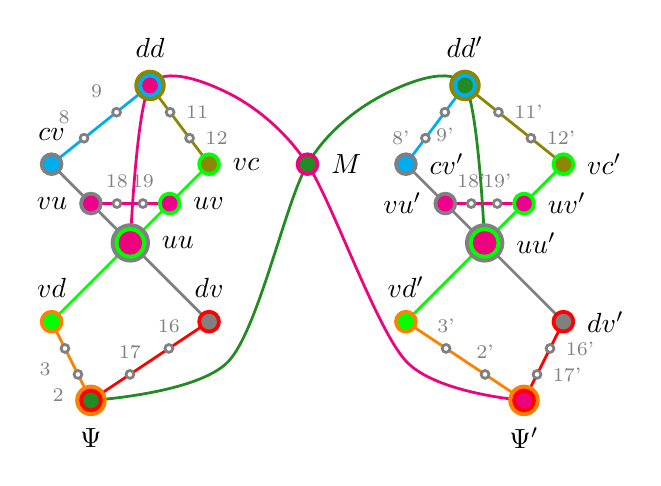
\begin{tikzpicture}  [scale=0.5]
        \tikzstyle{every path}=[line width=1pt]
        \newdimen\ms
        \ms=0.1cm
        \tikzstyle{s1}=[color=red,rectangle,inner sep=3.5]
        \tikzstyle{c4}=[circle,inner sep={\ms/8},minimum size=5*\ms]
        \tikzstyle{c3}=[circle,inner sep={\ms/8},minimum size=4*\ms]
        \tikzstyle{c2}=[circle,inner sep={\ms/8},minimum size=3*\ms]
        \tikzstyle{c1}=[circle,inner sep={\ms/8},minimum size=2*\ms]
        \tikzstyle{cs1}=[circle,inner sep={\ms/8},minimum size=1*\ms]

        \coordinate (psi) at (1,0);
        \coordinate (vd) at (0,2);
        \coordinate (dv) at (4,2);
        \coordinate (uu) at (2,4);
        \coordinate (vu) at (1,5);
        \coordinate (uv) at (3,5);
        \coordinate (cv) at (0,6);
        \coordinate (vc) at (4,6);
        \coordinate (dd) at (2.5,8);
        \coordinate (aux1) at (4.5,1);
        \coordinate (aux2) at (9,1);
        \coordinate (aux3) at (4.5,7.8);
        \coordinate (aux4) at (8.5,7.8);
        \coordinate (P) at (10.5,8);
        \coordinate (M) at (6.5,6);
        \coordinate (N) at (12,0);
        \coordinate (psi2) at ({3+9},0);
        \coordinate (vd2) at ({0+9},2);
        \coordinate (dv2) at ({4+9},2);
        \coordinate (uu2) at ({2+9},4);
        \coordinate (vu2) at ({1+9},5);
        \coordinate (uv2) at ({3+9},5);
        \coordinate (cv2) at ({0+9},6);
        \coordinate (vc2) at ({4+9},6);
        \coordinate (dd2) at ({1.5+9},8);

        \draw [color=orange] (psi) -- (vd)  coordinate[cs1,fill=white,draw=gray,pos=0.33,label=below left:{\scriptsize \color{gray}2}] (2)  coordinate[cs1,fill=white,draw=gray,pos=0.66,label=below left:{\scriptsize \color{gray}3}] (3);
        \draw [color=red] (psi) -- (dv) coordinate[cs1,fill=white,draw=gray,pos=0.33,label=above:{\scriptsize \color{gray}17}]  (17) coordinate[cs1,fill=white,draw=gray,pos=0.66,label=above:{\scriptsize \color{gray}16}] (16);
        \draw [color=green] (vd) -- (vc);
        \draw [color=gray] (dv) -- (cv);
        \draw [color=magenta] (vu) -- (uv) coordinate[cs1,fill=white,draw=gray,pos=0.33,label=above:{\scriptsize \color{gray}18}] (18)  coordinate[cs1,fill=white,draw=gray,pos=0.66,label=above:{\scriptsize \color{gray}19}] (19);
        \draw [color=cyan] (cv) -- (dd) coordinate[cs1,fill=white,draw=gray,pos=0.33,label=above left:{\scriptsize \color{gray}8}]  (8) coordinate[cs1,fill=white,draw=gray,pos=0.66,label=above left:{\scriptsize \color{gray}9}] (9);
        \draw [color=olive] (vc) -- (dd) coordinate[cs1,fill=white,draw=gray,pos=0.33,label=right:{\scriptsize \color{gray}12}] (12)  coordinate[cs1,fill=white,draw=gray,pos=0.66,label=right:{\scriptsize \color{gray}11}] (11);
        \draw [color=orange] (psi2) -- (vd2)  coordinate[cs1,fill=white,draw=gray,pos=0.33,label=above:{\scriptsize \color{gray}2'}] (22)  coordinate[cs1,fill=white,draw=gray,pos=0.66,label=above:{\scriptsize \color{gray}3'}] (32);
        \draw [color=red] (psi2) -- (dv2) coordinate[cs1,fill=white,draw=gray,pos=0.33,label=right:{\scriptsize \color{gray}17'}]  (172) coordinate[cs1,fill=white,draw=gray,pos=0.66,label=right:{\scriptsize \color{gray}16'}] (162);
        \draw [color=green] (vd2) -- (vc2);
        \draw [color=gray] (dv2) -- (cv2);
        \draw [color=magenta] (vu2) -- (uv2) coordinate[cs1,fill=white,draw=gray,pos=0.33,label=above:{\scriptsize \color{gray}18'}] (182)  coordinate[cs1,fill=white,draw=gray,pos=0.66,label=above:{\scriptsize \color{gray}19'}] (192);
        \draw [color=cyan] (cv2) -- (dd2) coordinate[cs1,fill=white,draw=gray,pos=0.33,label=left:{\scriptsize \color{gray}8'}]  (82) coordinate[cs1,fill=white,draw=gray,pos=0.66,label=below:{\scriptsize \color{gray}9'}] (92);
        \draw [color=olive] (vc2) -- (dd2) coordinate[cs1,fill=white,draw=gray,pos=0.33,label=right:{\scriptsize \color{gray}12'}] (122)  coordinate[cs1,fill=white,draw=gray,pos=0.66,label=right:{\scriptsize \color{gray}11'}] (112);

        \draw [ForestGreen] plot [smooth] coordinates {(psi)  (aux1) (M) (aux4) (P) (uu2) };
        \draw [RubineRed] plot [smooth] coordinates {(uu) (dd) (aux3) (M) (aux2) (N)};

        \draw (psi) coordinate[c3,fill=orange,label=below:$\Psi$];
        \draw (psi) coordinate[c2,fill=red];
        \draw (psi) coordinate[c1,fill=ForestGreen];
        \draw (vd) coordinate[c2,fill=orange,label=above:$vd$];
        \draw (vd) coordinate[c1,fill=green];
        \draw (dv) coordinate[c2,fill=red,label=above:$dv$];
        \draw (dv) coordinate[c1,fill=gray];
        \draw (uu) coordinate[c4,fill=gray,label=right:$uu$];
        \draw (uu) coordinate[c3,fill=green];
        \draw (uu) coordinate[c2,fill=RubineRed];
        \draw (vu) coordinate[c2,fill=gray,label=left:$vu$];
        \draw (vu) coordinate[c1,fill=magenta];
        \draw (uv) coordinate[c2,fill=green,label=right:$uv$];
        \draw (uv) coordinate[c1,fill=magenta];
        \draw (cv) coordinate[c2,fill=gray,label=above:$cv$];
        \draw (cv) coordinate[c1,fill=cyan];
        \draw (vc) coordinate[c2,fill=green,label=right:$vc$];
        \draw (vc) coordinate[c1,fill=olive];
        \draw (dd) coordinate[c3,fill=olive,label=above:$dd$];
        \draw (dd) coordinate[c2,fill=cyan];
        \draw (dd) coordinate[c1,fill=RubineRed];
        \draw (psi2) coordinate[c3,fill=orange,label=below:$\Psi'$];
        \draw (psi2) coordinate[c2,fill=red];
        \draw (psi2) coordinate[c1,fill=RubineRed];
        \draw (vd2) coordinate[c2,fill=orange,label=above:$vd'$];
        \draw (vd2) coordinate[c1,fill=green];
        \draw (dv2) coordinate[c2,fill=red,label=right:$dv'$];
        \draw (dv2) coordinate[c1,fill=gray];
        \draw (uu2) coordinate[c4,fill=gray,label=right:$uu'$];
        \draw (uu2) coordinate[c3,fill=green];
        \draw (uu2) coordinate[c2,fill=RubineRed];
        \draw (vu2) coordinate[c2,fill=gray,label=left:$vu'$];
        \draw (vu2) coordinate[c1,fill=magenta];
        \draw (uv2) coordinate[c2,fill=green,label=right:$uv'$];
        \draw (uv2) coordinate[c1,fill=magenta];
        \draw (cv2) coordinate[c2,fill=gray,label=right:$cv'$];
        \draw (cv2) coordinate[c1,fill=cyan];
        \draw (vc2) coordinate[c2,fill=green,label=right:$vc'$];
        \draw (vc2) coordinate[c1,fill=olive];
        \draw (dd2) coordinate[c3,fill=olive,label=above:$dd'$];
        \draw (dd2) coordinate[c2,fill=cyan];
        \draw (dd2) coordinate[c1,fill=ForestGreen];
        \draw (M) coordinate[c2,fill=RubineRed,label=right:$M$];
        \draw (M) coordinate[c1,fill=ForestGreen];
        \end{tikzpicture}
        }
        &
        \resizebox{.3\textwidth}{!}{%
        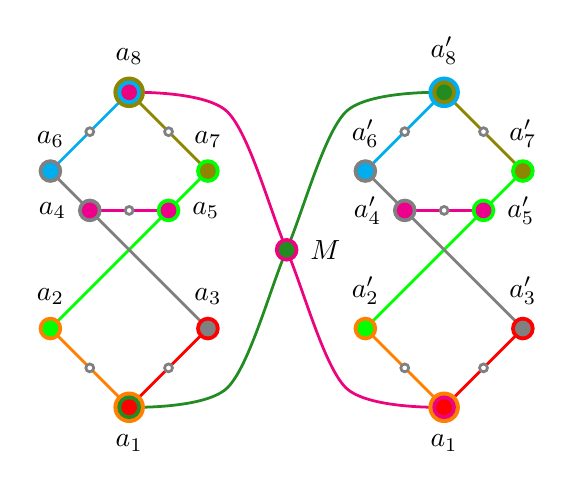
\begin{tikzpicture}  [scale=0.5]
        \tikzstyle{every path}=[line width=1pt]
        \newdimen\ms
        \ms=0.1cm
        \tikzstyle{s1}=[color=red,rectangle,inner sep=3.5]
        \tikzstyle{c3}=[circle,inner sep={\ms/8},minimum size=4*\ms]
        \tikzstyle{c2}=[circle,inner sep={\ms/8},minimum size=3*\ms]
        \tikzstyle{c1}=[circle,inner sep={\ms/8},minimum size=2*\ms]
        \tikzstyle{cs1}=[circle,inner sep={\ms/8},minimum size=1*\ms]

        \coordinate (a1) at (2,0);
        \coordinate (a2) at (0,2);
        \coordinate (a3) at (4,2);
        \coordinate (uu) at (2,4);
        \coordinate (a4) at (1,5);
        \coordinate (a5) at (3,5);
        \coordinate (a6) at (0,6);
        \coordinate (a7) at (4,6);
        \coordinate (a8) at (2,8);
        \coordinate (a12) at ({2+8},0);
        \coordinate (a22) at ({0+8},2);
        \coordinate (a32) at ({4+8},2);
        \coordinate (uu2) at ({2+8},4);
        \coordinate (a42) at ({1+8},5);
        \coordinate (a52) at ({3+8},5);
        \coordinate (a62) at ({0+8},6);
        \coordinate (a72) at ({4+8},6);
        \coordinate (a82) at ({2+8},8);
        \coordinate (O) at (10,8);
        \coordinate (M) at (6,4);
        \coordinate (N) at (10,0);
        \coordinate (aux1) at (4.5,0.5);
        \coordinate (aux2) at (4.5,7.5);
        \coordinate (aux12) at (7.5,0.5);
        \coordinate (aux22) at (7.5,7.5);

        \draw [color=orange] (a1) -- (a2)  coordinate[cs1,fill=white,draw=gray,pos=0.5] (2) ;
        \draw [color=red] (a1) -- (a3) coordinate[cs1,fill=white,draw=gray,pos=0.5]  (17);
        \draw [color=green] (a2) -- (a7);
        \draw [color=gray] (a3) -- (a6);
        \draw [color=magenta] (a4) -- (a5) coordinate[cs1,fill=white,draw=gray,pos=0.5] (18);
        \draw [color=cyan] (a6) -- (a8) coordinate[cs1,fill=white,draw=gray,pos=0.5]  (8);
        \draw [color=olive] (a7) -- (a8) coordinate[cs1,fill=white,draw=gray,pos=0.5] (12);
        \draw [color=orange!100!white] (a12) -- (a22)  coordinate[cs1,fill=white,draw=gray,pos=0.5] (2) ;
        \draw [color=red!100!white] (a12) -- (a32) coordinate[cs1,fill=white,draw=gray,pos=0.5]  (17);
        \draw [color=green!100!white] (a22) -- (a72);
        \draw [color=gray!100!white] (a32) -- (a62);
        \draw [color=magenta!100!white] (a42) -- (a52) coordinate[cs1,fill=white,draw=gray,pos=0.5] (18);
        \draw [color=cyan!100!white] (a62) -- (a82) coordinate[cs1,fill=white,draw=gray,pos=0.5]  (8);
        \draw [color=olive!100!white] (a72) -- (a82) coordinate[cs1,fill=white,draw=gray,pos=0.5] (12);

        \draw [ForestGreen] plot [smooth] coordinates {(a1) (aux1) (M) (aux22) (O)};
        \draw [RubineRed] plot [smooth] coordinates {(a8) (aux2) (M) (aux12) (N)};

        \draw (a1) coordinate[c3,fill=orange,label=below:$a_1$];
        \draw (a1) coordinate[c2,fill=ForestGreen];
        \draw (a1) coordinate[c1,fill=red];
        \draw (a2) coordinate[c2,fill=orange,label=above:$a_2$];
        \draw (a2) coordinate[c1,fill=green];
        \draw (a3) coordinate[c2,fill=red,label=above:$a_3$];
        \draw (a3) coordinate[c1,fill=gray];
        \draw (a4) coordinate[c2,fill=gray,label=left:$a_4$];
        \draw (a4) coordinate[c1,fill=magenta];
        \draw (a5) coordinate[c2,fill=green,label=right:$a_5$];
        \draw (a5) coordinate[c1,fill=magenta];
        \draw (a6) coordinate[c2,fill=gray,label=above:$a_6$];
        \draw (a6) coordinate[c1,fill=cyan];
        \draw (a7) coordinate[c2,fill=green,label=above:$a_7$];
        \draw (a7) coordinate[c1,fill=olive];
        \draw (a8) coordinate[c3,fill=olive,label=above:$a_8$];
        \draw (a8) coordinate[c2,fill=cyan];
        \draw (a8) coordinate[c1,fill=RubineRed];
        \draw (a12) coordinate[c3,fill=orange,label=below:$a_1$];
        \draw (a12) coordinate[c2,fill=RubineRed];
        \draw (a12) coordinate[c1,fill=red];
        \draw (a22) coordinate[c2,fill=orange,label=above:$a_2'$];
        \draw (a22) coordinate[c1,fill=green];
        \draw (a32) coordinate[c2,fill=red,label=above:$a_3'$];
        \draw (a32) coordinate[c1,fill=gray];
        \draw (a42) coordinate[c2,fill=gray,label=left:$a_4'$];
        \draw (a42) coordinate[c1,fill=magenta];
        \draw (a52) coordinate[c2,fill=green,label=right:$a_5'$];
        \draw (a52) coordinate[c1,fill=magenta];
        \draw (a62) coordinate[c2,fill=gray,label=above:$a_6'$];
        \draw (a62) coordinate[c1,fill=cyan];
        \draw (a72) coordinate[c2,fill=green,label=above:$a_7'$];
        \draw (a72) coordinate[c1,fill=olive];
        \draw (a82) coordinate[c3,fill=cyan,label=above:$a_8'$];
        \draw (a82) coordinate[c2,fill=olive];
        \draw (a82) coordinate[c1,fill=ForestGreen];
        \draw (M) coordinate[c2,fill=RubineRed,label=right:$M$];
        \draw (M) coordinate[c1,fill=ForestGreen];
        \end{tikzpicture}
        }
        \\
        (a)&(b)&(c)
        \\
        \resizebox{.35\textwidth}{!}{%
        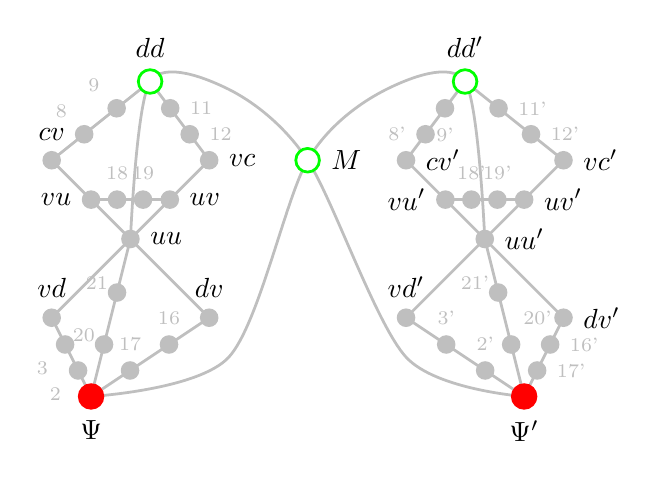
\begin{tikzpicture}  [scale=0.5]
        \tikzstyle{every path}=[line width=1pt]
        \newdimen\ms
        \ms=0.1cm
        \tikzstyle{s1}=[color=red,rectangle,inner sep=3.5]
        \tikzstyle{c4}=[circle,inner sep={\ms/8},minimum size=5*\ms]
        \tikzstyle{c3}=[circle,inner sep={\ms/8},minimum size=4*\ms]
        \tikzstyle{c2}=[circle,inner sep={\ms/8},minimum size=3*\ms]
        \tikzstyle{c1}=[circle,inner sep={\ms/8},minimum size=2*\ms]
        \tikzstyle{cs1}=[circle,inner sep={\ms/8},minimum size=1*\ms]

        \coordinate (psi) at (1,0);
        \coordinate (vd) at (0,2);
        \coordinate (dv) at (4,2);
        \coordinate (uu) at (2,4);
        \coordinate (vu) at (1,5);
        \coordinate (uv) at (3,5);
        \coordinate (cv) at (0,6);
        \coordinate (vc) at (4,6);
        \coordinate (dd) at (2.5,8);
        \coordinate (aux1) at (4.5,1);
        \coordinate (aux2) at (9,1);
        \coordinate (aux3) at (4.5,7.8);
        \coordinate (aux4) at (8.5,7.8);
        \coordinate (P) at (10.5,8);
        \coordinate (M) at (6.5,6);
        \coordinate (N) at (12,0);
        \coordinate (psi2) at ({3+9},0);
        \coordinate (vd2) at ({0+9},2);
        \coordinate (dv2) at ({4+9},2);
        \coordinate (uu2) at ({2+9},4);
        \coordinate (vu2) at ({1+9},5);
        \coordinate (uv2) at ({3+9},5);
        \coordinate (cv2) at ({0+9},6);
        \coordinate (vc2) at ({4+9},6);
        \coordinate (dd2) at ({1.5+9},8);

        \draw [color=lightgray] (psi) -- (vd)  coordinate[c1,fill=lightgray,draw=lightgray,pos=0.33,label=below left:{\scriptsize \color{lightgray}2}] (2)  coordinate[c1,fill=lightgray,draw=lightgray,pos=0.66,label=below left:{\scriptsize \color{lightgray}3}] (3);
        \draw [color=lightgray] (psi) -- (uu)  coordinate[c1,fill=lightgray,draw=lightgray,pos=0.33,label={[left,xshift=0.2mm]:{\scriptsize \color{lightgray}20}}] (20)  coordinate[c1,fill=lightgray,draw=lightgray,pos=0.66,label={[left,xshift=0.2mm]:{\scriptsize \color{lightgray}21}}] (21);
        \draw [color=lightgray] (psi) -- (dv) coordinate[c1,fill=lightgray,draw=lightgray,pos=0.33,label=above:{\scriptsize \color{lightgray}17}]  (17) coordinate[c1,fill=lightgray,draw=lightgray,pos=0.66,label=above:{\scriptsize \color{lightgray}16}] (16);
        \draw [color=lightgray] (vd) -- (vc);
        \draw [color=lightgray] (dv) -- (cv);
        \draw [color=lightgray] (vu) -- (uv) coordinate[c1,fill=lightgray,draw=lightgray,pos=0.33,label=above:{\scriptsize \color{lightgray}18}] (18)  coordinate[c1,fill=lightgray,draw=lightgray,pos=0.66,label=above:{\scriptsize \color{lightgray}19}] (19);
        \draw [color=lightgray] (cv) -- (dd) coordinate[c1,fill=lightgray,draw=lightgray,pos=0.33,label=above left:{\scriptsize \color{lightgray}8}]  (8) coordinate[c1,fill=lightgray,draw=lightgray,pos=0.66,label=above left:{\scriptsize \color{lightgray}9}] (9);
        \draw [color=lightgray] (vc) -- (dd) coordinate[c1,fill=lightgray,draw=lightgray,pos=0.33,label=right:{\scriptsize \color{lightgray}12}] (12)  coordinate[c1,fill=lightgray,draw=lightgray,pos=0.66,label=right:{\scriptsize \color{lightgray}11}] (11);
        \draw [color=lightgray] (psi2) -- (vd2)  coordinate[c1,fill=lightgray,draw=lightgray,pos=0.33,label=above:{\scriptsize \color{lightgray}2'}] (22)  coordinate[c1,fill=lightgray,draw=lightgray,pos=0.66,label=above:{\scriptsize \color{lightgray}3'}] (32);
        \draw [color=lightgray] (psi2) -- (uu2)  coordinate[c1,fill=lightgray,draw=lightgray,pos=0.33,label={[above right,xshift=0.2mm]:{\scriptsize \color{lightgray}20'}}] (202)  coordinate[c1,fill=lightgray,draw=lightgray,pos=0.66,label={[left,xshift=0.2mm]:{\scriptsize \color{lightgray}21'}}] (212);
        \draw [color=lightgray] (psi2) -- (dv2) coordinate[c1,fill=lightgray,draw=lightgray,pos=0.33,label=right:{\scriptsize \color{lightgray}17'}]  (172) coordinate[c1,fill=lightgray,draw=lightgray,pos=0.66,label=right:{\scriptsize \color{lightgray}16'}] (162);
        \draw [color=lightgray] (vd2) -- (vc2);
        \draw [color=lightgray] (dv2) -- (cv2);
        \draw [color=lightgray] (vu2) -- (uv2) coordinate[c1,fill=lightgray,draw=lightgray,pos=0.33,label=above:{\scriptsize \color{lightgray}18'}] (182)  coordinate[c1,fill=lightgray,draw=lightgray,pos=0.66,label=above:{\scriptsize \color{lightgray}19'}] (192);
        \draw [color=lightgray] (cv2) -- (dd2) coordinate[c1,fill=lightgray,draw=lightgray,pos=0.33,label=left:{\scriptsize \color{lightgray}8'}]  (82) coordinate[c1,fill=lightgray,draw=lightgray,pos=0.66,label=below:{\scriptsize \color{lightgray}9'}] (92);
        \draw [color=lightgray] (vc2) -- (dd2) coordinate[c1,fill=lightgray,draw=lightgray,pos=0.33,label=right:{\scriptsize \color{lightgray}12'}] (122)  coordinate[c1,fill=lightgray,draw=lightgray,pos=0.66,label=right:{\scriptsize \color{lightgray}11'}] (112);

        \draw [lightgray] plot [smooth] coordinates {(psi)  (aux1) (M) (aux4) (P) (uu2) };
        \draw [lightgray] plot [smooth] coordinates {(uu) (dd) (aux3) (M) (aux2) (N)};

        \draw (psi) coordinate[c2,fill=red,draw=red,label=below:$\Psi$];
        \draw (vd) coordinate[c1,fill=lightgray,draw=lightgray,label=above:$vd$];
        \draw (dv) coordinate[c1,fill=lightgray,draw=lightgray,label=above:$dv$];
        \draw (uu) coordinate[c1,fill=lightgray,draw=lightgray,label=right:$uu$];
        \draw (vu) coordinate[c1,fill=lightgray,draw=lightgray,label=left:$vu$];
        \draw (uv) coordinate[c1,fill=lightgray,draw=lightgray,label=right:$uv$];
        \draw (cv) coordinate[c1,fill=lightgray,draw=lightgray,label=above:$cv$];
        \draw (vc) coordinate[c1,fill=lightgray,draw=lightgray,label=right:$vc$];
        \draw (dd) coordinate[c2,fill=white,draw=green,label=above:$dd$];
        \draw (psi2) coordinate[c2,fill=red,draw=red,label=below:$\Psi'$];
        \draw (vd2) coordinate[c1,fill=lightgray,draw=lightgray,label=above:$vd'$];
        \draw (dv2) coordinate[c1,fill=lightgray,draw=lightgray,label=right:$dv'$];
        \draw (uu2) coordinate[c1,fill=lightgray,draw=lightgray,label=right:$uu'$];
        \draw (vu2) coordinate[c1,fill=lightgray,draw=lightgray,label=left:$vu'$];
        \draw (uv2) coordinate[c1,fill=lightgray,draw=lightgray,label=right:$uv'$];
        \draw (cv2) coordinate[c1,fill=lightgray,draw=lightgray,label=right:$cv'$];
        \draw (vc2) coordinate[c1,fill=lightgray,draw=lightgray,label=right:$vc'$];
        \draw (dd2) coordinate[c2,fill=white,draw=green,label=above:$dd'$];
        \draw (M) coordinate[c2,fill=white,draw=green,label=right:$M$];
        \end{tikzpicture}
        }
        &
        \resizebox{.35\textwidth}{!}{%
        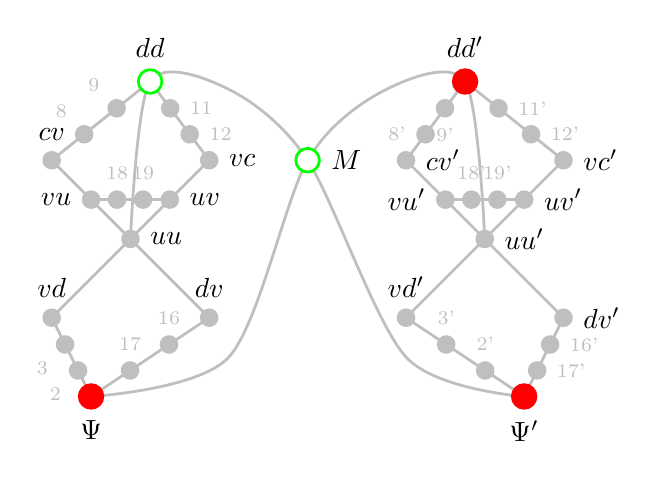
\begin{tikzpicture}  [scale=0.5]
        \tikzstyle{every path}=[line width=1pt]
        \newdimen\ms
        \ms=0.1cm
        \tikzstyle{s1}=[color=lightgray,rectangle,inner sep=3.5]
        \tikzstyle{c4}=[circle,inner sep={\ms/8},minimum size=5*\ms]
        \tikzstyle{c3}=[circle,inner sep={\ms/8},minimum size=4*\ms]
        \tikzstyle{c2}=[circle,inner sep={\ms/8},minimum size=3*\ms]
        \tikzstyle{c1}=[circle,inner sep={\ms/8},minimum size=2*\ms]
        \tikzstyle{cs1}=[circle,inner sep={\ms/8},minimum size=1*\ms]

        \coordinate (psi) at (1,0);
        \coordinate (vd) at (0,2);
        \coordinate (dv) at (4,2);
        \coordinate (uu) at (2,4);
        \coordinate (vu) at (1,5);
        \coordinate (uv) at (3,5);
        \coordinate (cv) at (0,6);
        \coordinate (vc) at (4,6);
        \coordinate (dd) at (2.5,8);
        \coordinate (aux1) at (4.5,1);
        \coordinate (aux2) at (9,1);
        \coordinate (aux3) at (4.5,7.8);
        \coordinate (aux4) at (8.5,7.8);
        \coordinate (P) at (10.5,8);
        \coordinate (M) at (6.5,6);
        \coordinate (N) at (12,0);
        \coordinate (psi2) at ({3+9},0);
        \coordinate (vd2) at ({0+9},2);
        \coordinate (dv2) at ({4+9},2);
        \coordinate (uu2) at ({2+9},4);
        \coordinate (vu2) at ({1+9},5);
        \coordinate (uv2) at ({3+9},5);
        \coordinate (cv2) at ({0+9},6);
        \coordinate (vc2) at ({4+9},6);
        \coordinate (dd2) at ({1.5+9},8);

        \draw [color=lightgray] (psi) -- (vd)  coordinate[c1,fill=lightgray,draw=lightgray,pos=0.33,label=below left:{\scriptsize \color{lightgray}2}] (2)  coordinate[c1,fill=lightgray,draw=lightgray,pos=0.66,label=below left:{\scriptsize \color{lightgray}3}] (3);
        \draw [color=lightgray] (psi) -- (dv) coordinate[c1,fill=lightgray,draw=lightgray,pos=0.33,label=above:{\scriptsize \color{lightgray}17}]  (17) coordinate[c1,fill=lightgray,draw=lightgray,pos=0.66,label=above:{\scriptsize \color{lightgray}16}] (16);
        \draw [color=lightgray] (vd) -- (vc);
        \draw [color=lightgray] (dv) -- (cv);
        \draw [color=lightgray] (vu) -- (uv) coordinate[c1,fill=lightgray,draw=lightgray,pos=0.33,label=above:{\scriptsize \color{lightgray}18}] (18)  coordinate[c1,fill=lightgray,draw=lightgray,pos=0.66,label=above:{\scriptsize \color{lightgray}19}] (19);
        \draw [color=lightgray] (cv) -- (dd) coordinate[c1,fill=lightgray,draw=lightgray,pos=0.33,label=above left:{\scriptsize \color{lightgray}8}]  (8) coordinate[c1,fill=lightgray,draw=lightgray,pos=0.66,label=above left:{\scriptsize \color{lightgray}9}] (9);
        \draw [color=lightgray] (vc) -- (dd) coordinate[c1,fill=lightgray,draw=lightgray,pos=0.33,label=right:{\scriptsize \color{lightgray}12}] (12)  coordinate[c1,fill=lightgray,draw=lightgray,pos=0.66,label=right:{\scriptsize \color{lightgray}11}] (11);
        \draw [color=lightgray] (psi2) -- (vd2)  coordinate[c1,fill=lightgray,draw=lightgray,pos=0.33,label=above:{\scriptsize \color{lightgray}2'}] (22)  coordinate[c1,fill=lightgray,draw=lightgray,pos=0.66,label=above:{\scriptsize \color{lightgray}3'}] (32);
        \draw [color=lightgray] (psi2) -- (dv2) coordinate[c1,fill=lightgray,draw=lightgray,pos=0.33,label=right:{\scriptsize \color{lightgray}17'}]  (172) coordinate[c1,fill=lightgray,draw=lightgray,pos=0.66,label=right:{\scriptsize \color{lightgray}16'}] (162);
        \draw [color=lightgray] (vd2) -- (vc2);
        \draw [color=lightgray] (dv2) -- (cv2);
        \draw [color=lightgray] (vu2) -- (uv2) coordinate[c1,fill=lightgray,draw=lightgray,pos=0.33,label=above:{\scriptsize \color{lightgray}18'}] (182)  coordinate[c1,fill=lightgray,draw=lightgray,pos=0.66,label=above:{\scriptsize \color{lightgray}19'}] (192);
        \draw [color=lightgray] (cv2) -- (dd2) coordinate[c1,fill=lightgray,draw=lightgray,pos=0.33,label=left:{\scriptsize \color{lightgray}8'}]  (82) coordinate[c1,fill=lightgray,draw=lightgray,pos=0.66,label=below:{\scriptsize \color{lightgray}9'}] (92);
        \draw [color=lightgray] (vc2) -- (dd2) coordinate[c1,fill=lightgray,draw=lightgray,pos=0.33,label=right:{\scriptsize \color{lightgray}12'}] (122)  coordinate[c1,fill=lightgray,draw=lightgray,pos=0.66,label=right:{\scriptsize \color{lightgray}11'}] (112);

        \draw [lightgray] plot [smooth] coordinates {(psi)  (aux1) (M) (aux4) (P) (uu2) };
        \draw [lightgray] plot [smooth] coordinates {(uu) (dd) (aux3) (M) (aux2) (N)};

        \draw (psi) coordinate[c2,fill=red,draw=red,label=below:$\Psi$];
        \draw (vd) coordinate[c1,fill=lightgray,draw=lightgray,label=above:$vd$];
        \draw (dv) coordinate[c1,fill=lightgray,draw=lightgray,label=above:$dv$];
        \draw (uu) coordinate[c1,fill=lightgray,draw=lightgray,label=right:$uu$];
        \draw (vu) coordinate[c1,fill=lightgray,draw=lightgray,label=left:$vu$];
        \draw (uv) coordinate[c1,fill=lightgray,draw=lightgray,label=right:$uv$];
        \draw (cv) coordinate[c1,fill=lightgray,draw=lightgray,label=above:$cv$];
        \draw (vc) coordinate[c1,fill=lightgray,draw=lightgray,label=right:$vc$];
        \draw (dd) coordinate[c2,fill=white,draw=green,label=above:$dd$];
        \draw (psi2) coordinate[c2,fill=red,draw=red,label=below:$\Psi'$];
        \draw (vd2) coordinate[c1,fill=lightgray,draw=lightgray,label=above:$vd'$];
        \draw (dv2) coordinate[c1,fill=lightgray,draw=lightgray,label=right:$dv'$];
        \draw (uu2) coordinate[c1,fill=lightgray,draw=lightgray,label=right:$uu'$];
        \draw (vu2) coordinate[c1,fill=lightgray,draw=lightgray,label=left:$vu'$];
        \draw (uv2) coordinate[c1,fill=lightgray,draw=lightgray,label=right:$uv'$];
        \draw (cv2) coordinate[c1,fill=lightgray,draw=lightgray,label=right:$cv'$];
        \draw (vc2) coordinate[c1,fill=lightgray,draw=lightgray,label=right:$vc'$];
        \draw (dd2) coordinate[c2,fill=red,draw=red,label=above:$dd'$];
        \draw (M) coordinate[c2,fill=white,draw=green,label=right:$M$];
        \end{tikzpicture}
        }
        &
        \resizebox{.3\textwidth}{!}{%
        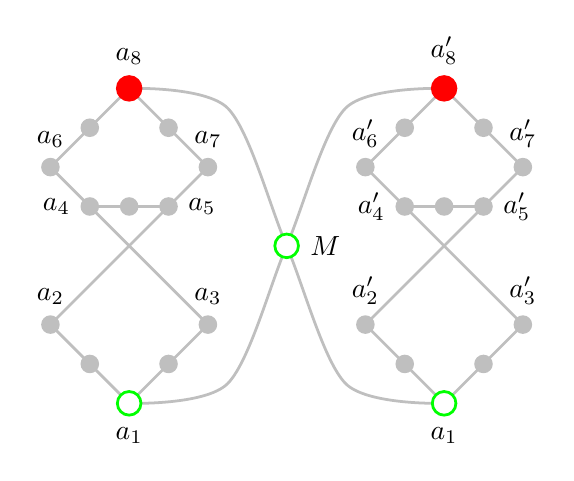
\begin{tikzpicture}  [scale=0.5]
        \tikzstyle{every path}=[line width=1pt]
        \newdimen\ms
        \ms=0.1cm
        \tikzstyle{s1}=[color=lightgray,rectangle,inner sep=3.5]
        \tikzstyle{c3}=[circle,inner sep={\ms/8},minimum size=4*\ms]
        \tikzstyle{c2}=[circle,inner sep={\ms/8},minimum size=3*\ms]
        \tikzstyle{c1}=[circle,inner sep={\ms/8},minimum size=2*\ms]
        \tikzstyle{cs1}=[circle,inner sep={\ms/8},minimum size=1*\ms]

        \coordinate (a1) at (2,0);
        \coordinate (a2) at (0,2);
        \coordinate (a3) at (4,2);
        \coordinate (uu) at (2,4);
        \coordinate (a4) at (1,5);
        \coordinate (a5) at (3,5);
        \coordinate (a6) at (0,6);
        \coordinate (a7) at (4,6);
        \coordinate (a8) at (2,8);
        \coordinate (a12) at ({2+8},0);
        \coordinate (a22) at ({0+8},2);
        \coordinate (a32) at ({4+8},2);
        \coordinate (uu2) at ({2+8},4);
        \coordinate (a42) at ({1+8},5);
        \coordinate (a52) at ({3+8},5);
        \coordinate (a62) at ({0+8},6);
        \coordinate (a72) at ({4+8},6);
        \coordinate (a82) at ({2+8},8);
        \coordinate (O) at (10,8);
        \coordinate (M) at (6,4);
        \coordinate (N) at (10,0);
        \coordinate (aux1) at (4.5,0.5);
        \coordinate (aux2) at (4.5,7.5);
        \coordinate (aux12) at (7.5,0.5);
        \coordinate (aux22) at (7.5,7.5);

        \draw [color=lightgray] (a1) -- (a2)  coordinate[c1,fill=lightgray,draw=lightgray,pos=0.5] (2) ;
        \draw [color=lightgray] (a1) -- (a3) coordinate[c1,fill=lightgray,draw=lightgray,pos=0.5]  (17);
        \draw [color=lightgray] (a2) -- (a7);
        \draw [color=lightgray] (a3) -- (a6);
        \draw [color=lightgray] (a4) -- (a5) coordinate[c1,fill=lightgray,draw=lightgray,pos=0.5] (18);
        \draw [color=lightgray] (a6) -- (a8) coordinate[c1,fill=lightgray,draw=lightgray,pos=0.5]  (8);
        \draw [color=lightgray] (a7) -- (a8) coordinate[c1,fill=lightgray,draw=lightgray,pos=0.5] (12);
        \draw [color=lightgray!100!white] (a12) -- (a22)  coordinate[c1,fill=lightgray,draw=lightgray,pos=0.5] (2) ;
        \draw [color=lightgray!100!white] (a12) -- (a32) coordinate[c1,fill=lightgray,draw=lightgray,pos=0.5]  (17);
        \draw [color=lightgray!100!white] (a22) -- (a72);
        \draw [color=lightgray!100!white] (a32) -- (a62);
        \draw [color=lightgray!100!white] (a42) -- (a52) coordinate[c1,fill=lightgray,draw=lightgray,pos=0.5] (18);
        \draw [color=lightgray!100!white] (a62) -- (a82) coordinate[c1,fill=lightgray,draw=lightgray,pos=0.5]  (8);
        \draw [color=lightgray!100!white] (a72) -- (a82) coordinate[c1,fill=lightgray,draw=lightgray,pos=0.5] (12);

        \draw [lightgray] plot [smooth] coordinates {(a1) (aux1) (M) (aux22) (O)};
        \draw [lightgray] plot [smooth] coordinates {(a8) (aux2) (M) (aux12) (N)};

        \draw (a1) coordinate[c2,fill=white,draw=green,label=below:$a_1$];
        \draw (a2) coordinate[c1,fill=lightgray,draw=lightgray,label=above:$a_2$];
        \draw (a3) coordinate[c1,fill=lightgray,draw=lightgray,label=above:$a_3$];
        \draw (a4) coordinate[c1,fill=lightgray,draw=lightgray,label=left:$a_4$];
        \draw (a5) coordinate[c1,fill=lightgray,draw=lightgray,label=right:$a_5$];
        \draw (a6) coordinate[c1,fill=lightgray,draw=lightgray,label=above:$a_6$];
        \draw (a7) coordinate[c1,fill=lightgray,draw=lightgray,label=above:$a_7$];
        \draw (a8) coordinate[c2,fill=red,draw=red,label=above:$a_8$];
        \draw (a12) coordinate[c2,fill=white,draw=green,label=below:$a_1$];
        \draw (a22) coordinate[c1,fill=lightgray,draw=lightgray,label=above:$a_2'$];
        \draw (a32) coordinate[c1,fill=lightgray,draw=lightgray,label=above:$a_3'$];
        \draw (a42) coordinate[c1,fill=lightgray,draw=lightgray,label=left:$a_4'$];
        \draw (a52) coordinate[c1,fill=lightgray,draw=lightgray,label=right:$a_5'$];
        \draw (a62) coordinate[c1,fill=lightgray,draw=lightgray,label=above:$a_6'$];
        \draw (a72) coordinate[c1,fill=lightgray,draw=lightgray,label=above:$a_7'$];
        \draw (a82) coordinate[c2,fill=red,draw=red,label=above:$a_8'$];
        \draw (M) coordinate[c2,fill=white,draw=green,label=right:$M$];
        \end{tikzpicture}
        }
        \\
        (d)&(e)&(f)\\
        \resizebox{.35\textwidth}{!}{%
        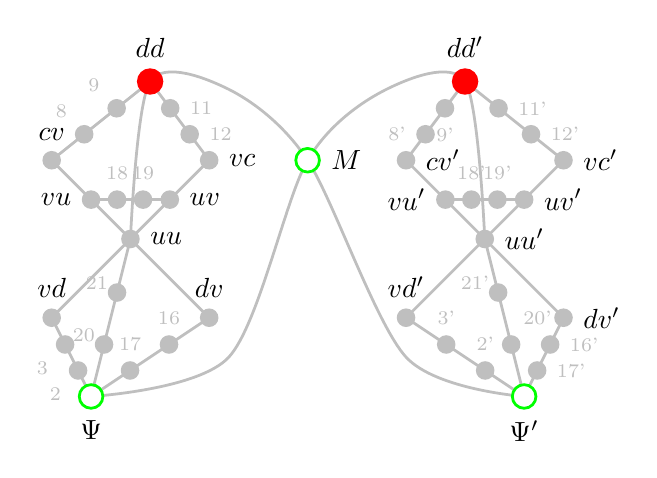
\begin{tikzpicture}  [scale=0.5]
        \tikzstyle{every path}=[line width=1pt]
        \newdimen\ms
        \ms=0.1cm
        \tikzstyle{s1}=[color=red,rectangle,inner sep=3.5]
        \tikzstyle{c4}=[circle,inner sep={\ms/8},minimum size=5*\ms]
        \tikzstyle{c3}=[circle,inner sep={\ms/8},minimum size=4*\ms]
        \tikzstyle{c2}=[circle,inner sep={\ms/8},minimum size=3*\ms]
        \tikzstyle{c1}=[circle,inner sep={\ms/8},minimum size=2*\ms]
        \tikzstyle{cs1}=[circle,inner sep={\ms/8},minimum size=1*\ms]

        \coordinate (psi) at (1,0);
        \coordinate (vd) at (0,2);
        \coordinate (dv) at (4,2);
        \coordinate (uu) at (2,4);
        \coordinate (vu) at (1,5);
        \coordinate (uv) at (3,5);
        \coordinate (cv) at (0,6);
        \coordinate (vc) at (4,6);
        \coordinate (dd) at (2.5,8);
        \coordinate (aux1) at (4.5,1);
        \coordinate (aux2) at (9,1);
        \coordinate (aux3) at (4.5,7.8);
        \coordinate (aux4) at (8.5,7.8);
        \coordinate (P) at (10.5,8);
        \coordinate (M) at (6.5,6);
        \coordinate (N) at (12,0);
        \coordinate (psi2) at ({3+9},0);
        \coordinate (vd2) at ({0+9},2);
        \coordinate (dv2) at ({4+9},2);
        \coordinate (uu2) at ({2+9},4);
        \coordinate (vu2) at ({1+9},5);
        \coordinate (uv2) at ({3+9},5);
        \coordinate (cv2) at ({0+9},6);
        \coordinate (vc2) at ({4+9},6);
        \coordinate (dd2) at ({1.5+9},8);

        \draw [color=lightgray] (psi) -- (vd)  coordinate[c1,fill=lightgray,draw=lightgray,pos=0.33,label=below left:{\scriptsize \color{lightgray}2}] (2)  coordinate[c1,fill=lightgray,draw=lightgray,pos=0.66,label=below left:{\scriptsize \color{lightgray}3}] (3);
        \draw [color=lightgray] (psi) -- (uu)  coordinate[c1,fill=lightgray,draw=lightgray,pos=0.33,label={[left,xshift=0.2mm]:{\scriptsize \color{lightgray}20}}] (20)  coordinate[c1,fill=lightgray,draw=lightgray,pos=0.66,label={[left,xshift=0.2mm]:{\scriptsize \color{lightgray}21}}] (21);
        \draw [color=lightgray] (psi) -- (dv) coordinate[c1,fill=lightgray,draw=lightgray,pos=0.33,label=above:{\scriptsize \color{lightgray}17}]  (17) coordinate[c1,fill=lightgray,draw=lightgray,pos=0.66,label=above:{\scriptsize \color{lightgray}16}] (16);
        \draw [color=lightgray] (vd) -- (vc);
        \draw [color=lightgray] (dv) -- (cv);
        \draw [color=lightgray] (vu) -- (uv) coordinate[c1,fill=lightgray,draw=lightgray,pos=0.33,label=above:{\scriptsize \color{lightgray}18}] (18)  coordinate[c1,fill=lightgray,draw=lightgray,pos=0.66,label=above:{\scriptsize \color{lightgray}19}] (19);
        \draw [color=lightgray] (cv) -- (dd) coordinate[c1,fill=lightgray,draw=lightgray,pos=0.33,label=above left:{\scriptsize \color{lightgray}8}]  (8) coordinate[c1,fill=lightgray,draw=lightgray,pos=0.66,label=above left:{\scriptsize \color{lightgray}9}] (9);
        \draw [color=lightgray] (vc) -- (dd) coordinate[c1,fill=lightgray,draw=lightgray,pos=0.33,label=right:{\scriptsize \color{lightgray}12}] (12)  coordinate[c1,fill=lightgray,draw=lightgray,pos=0.66,label=right:{\scriptsize \color{lightgray}11}] (11);
        \draw [color=lightgray] (psi2) -- (vd2)  coordinate[c1,fill=lightgray,draw=lightgray,pos=0.33,label=above:{\scriptsize \color{lightgray}2'}] (22)  coordinate[c1,fill=lightgray,draw=lightgray,pos=0.66,label=above:{\scriptsize \color{lightgray}3'}] (32);
        \draw [color=lightgray] (psi2) -- (uu2)  coordinate[c1,fill=lightgray,draw=lightgray,pos=0.33,label={[above right,xshift=0.2mm]:{\scriptsize \color{lightgray}20'}}] (202)  coordinate[c1,fill=lightgray,draw=lightgray,pos=0.66,label={[left,xshift=0.2mm]:{\scriptsize \color{lightgray}21'}}] (212);
        \draw [color=lightgray] (psi2) -- (dv2) coordinate[c1,fill=lightgray,draw=lightgray,pos=0.33,label=right:{\scriptsize \color{lightgray}17'}]  (172) coordinate[c1,fill=lightgray,draw=lightgray,pos=0.66,label=right:{\scriptsize \color{lightgray}16'}] (162);
        \draw [color=lightgray] (vd2) -- (vc2);
        \draw [color=lightgray] (dv2) -- (cv2);
        \draw [color=lightgray] (vu2) -- (uv2) coordinate[c1,fill=lightgray,draw=lightgray,pos=0.33,label=above:{\scriptsize \color{lightgray}18'}] (182)  coordinate[c1,fill=lightgray,draw=lightgray,pos=0.66,label=above:{\scriptsize \color{lightgray}19'}] (192);
        \draw [color=lightgray] (cv2) -- (dd2) coordinate[c1,fill=lightgray,draw=lightgray,pos=0.33,label=left:{\scriptsize \color{lightgray}8'}]  (82) coordinate[c1,fill=lightgray,draw=lightgray,pos=0.66,label=below:{\scriptsize \color{lightgray}9'}] (92);
        \draw [color=lightgray] (vc2) -- (dd2) coordinate[c1,fill=lightgray,draw=lightgray,pos=0.33,label=right:{\scriptsize \color{lightgray}12'}] (122)  coordinate[c1,fill=lightgray,draw=lightgray,pos=0.66,label=right:{\scriptsize \color{lightgray}11'}] (112);

        \draw [lightgray] plot [smooth] coordinates {(psi)  (aux1) (M) (aux4) (P) (uu2) };
        \draw [lightgray] plot [smooth] coordinates {(uu) (dd) (aux3) (M) (aux2) (N)};

        \draw (psi) coordinate[c2,fill=white,draw=green,label=below:$\Psi$];
        \draw (vd) coordinate[c1,fill=lightgray,draw=lightgray,label=above:$vd$];
        \draw (dv) coordinate[c1,fill=lightgray,draw=lightgray,label=above:$dv$];
        \draw (uu) coordinate[c1,fill=lightgray,draw=lightgray,label=right:$uu$];
        \draw (vu) coordinate[c1,fill=lightgray,draw=lightgray,label=left:$vu$];
        \draw (uv) coordinate[c1,fill=lightgray,draw=lightgray,label=right:$uv$];
        \draw (cv) coordinate[c1,fill=lightgray,draw=lightgray,label=above:$cv$];
        \draw (vc) coordinate[c1,fill=lightgray,draw=lightgray,label=right:$vc$];
        \draw (dd) coordinate[c2,fill=red,draw=red,label=above:$dd$];
        \draw (psi2) coordinate[c2,fill=white,draw=green,label=below:$\Psi'$];
        \draw (vd2) coordinate[c1,fill=lightgray,draw=lightgray,label=above:$vd'$];
        \draw (dv2) coordinate[c1,fill=lightgray,draw=lightgray,label=right:$dv'$];
        \draw (uu2) coordinate[c1,fill=lightgray,draw=lightgray,label=right:$uu'$];
        \draw (vu2) coordinate[c1,fill=lightgray,draw=lightgray,label=left:$vu'$];
        \draw (uv2) coordinate[c1,fill=lightgray,draw=lightgray,label=right:$uv'$];
        \draw (cv2) coordinate[c1,fill=lightgray,draw=lightgray,label=right:$cv'$];
        \draw (vc2) coordinate[c1,fill=lightgray,draw=lightgray,label=right:$vc'$];
        \draw (dd2) coordinate[c2,fill=red,draw=red,label=above:$dd'$];
        \draw (M) coordinate[c2,fill=white,draw=green,label=right:$M$];
        \end{tikzpicture}
        }
        &
        \resizebox{.35\textwidth}{!}{%
        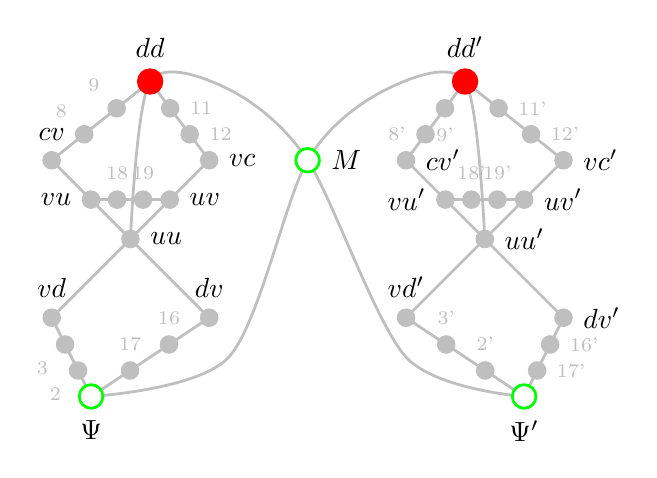
\begin{tikzpicture}  [scale=0.5]
        \tikzstyle{every path}=[line width=1pt]
        \newdimen\ms
        \ms=0.1cm
        \tikzstyle{s1}=[color=lightgray,rectangle,inner sep=3.5]
        \tikzstyle{c4}=[circle,inner sep={\ms/8},minimum size=5*\ms]
        \tikzstyle{c3}=[circle,inner sep={\ms/8},minimum size=4*\ms]
        \tikzstyle{c2}=[circle,inner sep={\ms/8},minimum size=3*\ms]
        \tikzstyle{c1}=[circle,inner sep={\ms/8},minimum size=2*\ms]
        \tikzstyle{cs1}=[circle,inner sep={\ms/8},minimum size=1*\ms]

        \coordinate (psi) at (1,0);
        \coordinate (vd) at (0,2);
        \coordinate (dv) at (4,2);
        \coordinate (uu) at (2,4);
        \coordinate (vu) at (1,5);
        \coordinate (uv) at (3,5);
        \coordinate (cv) at (0,6);
        \coordinate (vc) at (4,6);
        \coordinate (dd) at (2.5,8);
        \coordinate (aux1) at (4.5,1);
        \coordinate (aux2) at (9,1);
        \coordinate (aux3) at (4.5,7.8);
        \coordinate (aux4) at (8.5,7.8);
        \coordinate (P) at (10.5,8);
        \coordinate (M) at (6.5,6);
        \coordinate (N) at (12,0);
        \coordinate (psi2) at ({3+9},0);
        \coordinate (vd2) at ({0+9},2);
        \coordinate (dv2) at ({4+9},2);
        \coordinate (uu2) at ({2+9},4);
        \coordinate (vu2) at ({1+9},5);
        \coordinate (uv2) at ({3+9},5);
        \coordinate (cv2) at ({0+9},6);
        \coordinate (vc2) at ({4+9},6);
        \coordinate (dd2) at ({1.5+9},8);

        \draw [color=lightgray] (psi) -- (vd)  coordinate[c1,fill=lightgray,draw=lightgray,pos=0.33,label=below left:{\scriptsize \color{lightgray}2}] (2)  coordinate[c1,fill=lightgray,draw=lightgray,pos=0.66,label=below left:{\scriptsize \color{lightgray}3}] (3);
        \draw [color=lightgray] (psi) -- (dv) coordinate[c1,fill=lightgray,draw=lightgray,pos=0.33,label=above:{\scriptsize \color{lightgray}17}]  (17) coordinate[c1,fill=lightgray,draw=lightgray,pos=0.66,label=above:{\scriptsize \color{lightgray}16}] (16);
        \draw [color=lightgray] (vd) -- (vc);
        \draw [color=lightgray] (dv) -- (cv);
        \draw [color=lightgray] (vu) -- (uv) coordinate[c1,fill=lightgray,draw=lightgray,pos=0.33,label=above:{\scriptsize \color{lightgray}18}] (18)  coordinate[c1,fill=lightgray,draw=lightgray,pos=0.66,label=above:{\scriptsize \color{lightgray}19}] (19);
        \draw [color=lightgray] (cv) -- (dd) coordinate[c1,fill=lightgray,draw=lightgray,pos=0.33,label=above left:{\scriptsize \color{lightgray}8}]  (8) coordinate[c1,fill=lightgray,draw=lightgray,pos=0.66,label=above left:{\scriptsize \color{lightgray}9}] (9);
        \draw [color=lightgray] (vc) -- (dd) coordinate[c1,fill=lightgray,draw=lightgray,pos=0.33,label=right:{\scriptsize \color{lightgray}12}] (12)  coordinate[c1,fill=lightgray,draw=lightgray,pos=0.66,label=right:{\scriptsize \color{lightgray}11}] (11);
        \draw [color=lightgray] (psi2) -- (vd2)  coordinate[c1,fill=lightgray,draw=lightgray,pos=0.33,label=above:{\scriptsize \color{lightgray}2'}] (22)  coordinate[c1,fill=lightgray,draw=lightgray,pos=0.66,label=above:{\scriptsize \color{lightgray}3'}] (32);
        \draw [color=lightgray] (psi2) -- (dv2) coordinate[c1,fill=lightgray,draw=lightgray,pos=0.33,label=right:{\scriptsize \color{lightgray}17'}]  (172) coordinate[c1,fill=lightgray,draw=lightgray,pos=0.66,label=right:{\scriptsize \color{lightgray}16'}] (162);
        \draw [color=lightgray] (vd2) -- (vc2);
        \draw [color=lightgray] (dv2) -- (cv2);
        \draw [color=lightgray] (vu2) -- (uv2) coordinate[c1,fill=lightgray,draw=lightgray,pos=0.33,label=above:{\scriptsize \color{lightgray}18'}] (182)  coordinate[c1,fill=lightgray,draw=lightgray,pos=0.66,label=above:{\scriptsize \color{lightgray}19'}] (192);
        \draw [color=lightgray] (cv2) -- (dd2) coordinate[c1,fill=lightgray,draw=lightgray,pos=0.33,label=left:{\scriptsize \color{lightgray}8'}]  (82) coordinate[c1,fill=lightgray,draw=lightgray,pos=0.66,label=below:{\scriptsize \color{lightgray}9'}] (92);
        \draw [color=lightgray] (vc2) -- (dd2) coordinate[c1,fill=lightgray,draw=lightgray,pos=0.33,label=right:{\scriptsize \color{lightgray}12'}] (122)  coordinate[c1,fill=lightgray,draw=lightgray,pos=0.66,label=right:{\scriptsize \color{lightgray}11'}] (112);

        \draw [lightgray] plot [smooth] coordinates {(psi)  (aux1) (M) (aux4) (P) (uu2) };
        \draw [lightgray] plot [smooth] coordinates {(uu) (dd) (aux3) (M) (aux2) (N)};

        \draw (psi) coordinate[c2,fill=white,draw=green,label=below:$\Psi$];
        \draw (vd) coordinate[c1,fill=lightgray,draw=lightgray,label=above:$vd$];
        \draw (dv) coordinate[c1,fill=lightgray,draw=lightgray,label=above:$dv$];
        \draw (uu) coordinate[c1,fill=lightgray,draw=lightgray,label=right:$uu$];
        \draw (vu) coordinate[c1,fill=lightgray,draw=lightgray,label=left:$vu$];
        \draw (uv) coordinate[c1,fill=lightgray,draw=lightgray,label=right:$uv$];
        \draw (cv) coordinate[c1,fill=lightgray,draw=lightgray,label=above:$cv$];
        \draw (vc) coordinate[c1,fill=lightgray,draw=lightgray,label=right:$vc$];
        \draw (dd) coordinate[c2,fill=red,draw=red,label=above:$dd$];
        \draw (psi2) coordinate[c2,fill=white,draw=green,label=below:$\Psi'$];
        \draw (vd2) coordinate[c1,fill=lightgray,draw=lightgray,label=above:$vd'$];
        \draw (dv2) coordinate[c1,fill=lightgray,draw=lightgray,label=right:$dv'$];
        \draw (uu2) coordinate[c1,fill=lightgray,draw=lightgray,label=right:$uu'$];
        \draw (vu2) coordinate[c1,fill=lightgray,draw=lightgray,label=left:$vu'$];
        \draw (uv2) coordinate[c1,fill=lightgray,draw=lightgray,label=right:$uv'$];
        \draw (cv2) coordinate[c1,fill=lightgray,draw=lightgray,label=right:$cv'$];
        \draw (vc2) coordinate[c1,fill=lightgray,draw=lightgray,label=right:$vc'$];
        \draw (dd2) coordinate[c2,fill=red,draw=red,label=above:$dd'$];
        \draw (M) coordinate[c2,fill=white,draw=green,label=right:$M$];
        \end{tikzpicture}
        }
        &
        \resizebox{.3\textwidth}{!}{%
        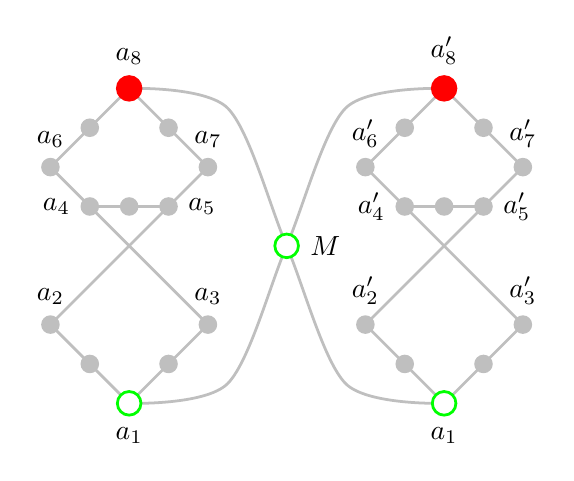
\begin{tikzpicture}  [scale=0.5]
        \tikzstyle{every path}=[line width=1pt]
        \newdimen\ms
        \ms=0.1cm
        \tikzstyle{s1}=[color=lightgray,rectangle,inner sep=3.5]
        \tikzstyle{c3}=[circle,inner sep={\ms/8},minimum size=4*\ms]
        \tikzstyle{c2}=[circle,inner sep={\ms/8},minimum size=3*\ms]
        \tikzstyle{c1}=[circle,inner sep={\ms/8},minimum size=2*\ms]
        \tikzstyle{cs1}=[circle,inner sep={\ms/8},minimum size=1*\ms]

        \coordinate (a1) at (2,0);
        \coordinate (a2) at (0,2);
        \coordinate (a3) at (4,2);
        \coordinate (uu) at (2,4);
        \coordinate (a4) at (1,5);
        \coordinate (a5) at (3,5);
        \coordinate (a6) at (0,6);
        \coordinate (a7) at (4,6);
        \coordinate (a8) at (2,8);
        \coordinate (a12) at ({2+8},0);
        \coordinate (a22) at ({0+8},2);
        \coordinate (a32) at ({4+8},2);
        \coordinate (uu2) at ({2+8},4);
        \coordinate (a42) at ({1+8},5);
        \coordinate (a52) at ({3+8},5);
        \coordinate (a62) at ({0+8},6);
        \coordinate (a72) at ({4+8},6);
        \coordinate (a82) at ({2+8},8);
        \coordinate (O) at (10,8);
        \coordinate (M) at (6,4);
        \coordinate (N) at (10,0);
        \coordinate (aux1) at (4.5,0.5);
        \coordinate (aux2) at (4.5,7.5);
        \coordinate (aux12) at (7.5,0.5);
        \coordinate (aux22) at (7.5,7.5);

        \draw [color=lightgray] (a1) -- (a2)  coordinate[c1,fill=lightgray,draw=lightgray,pos=0.5] (2) ;
        \draw [color=lightgray] (a1) -- (a3) coordinate[c1,fill=lightgray,draw=lightgray,pos=0.5]  (17);
        \draw [color=lightgray] (a2) -- (a7);
        \draw [color=lightgray] (a3) -- (a6);
        \draw [color=lightgray] (a4) -- (a5) coordinate[c1,fill=lightgray,draw=lightgray,pos=0.5] (18);
        \draw [color=lightgray] (a6) -- (a8) coordinate[c1,fill=lightgray,draw=lightgray,pos=0.5]  (8);
        \draw [color=lightgray] (a7) -- (a8) coordinate[c1,fill=lightgray,draw=lightgray,pos=0.5] (12);
        \draw [color=lightgray!100!white] (a12) -- (a22)  coordinate[c1,fill=lightgray,draw=lightgray,pos=0.5] (2) ;
        \draw [color=lightgray!100!white] (a12) -- (a32) coordinate[c1,fill=lightgray,draw=lightgray,pos=0.5]  (17);
        \draw [color=lightgray!100!white] (a22) -- (a72);
        \draw [color=lightgray!100!white] (a32) -- (a62);
        \draw [color=lightgray!100!white] (a42) -- (a52) coordinate[c1,fill=lightgray,draw=lightgray,pos=0.5] (18);
        \draw [color=lightgray!100!white] (a62) -- (a82) coordinate[c1,fill=lightgray,draw=lightgray,pos=0.5]  (8);
        \draw [color=lightgray!100!white] (a72) -- (a82) coordinate[c1,fill=lightgray,draw=lightgray,pos=0.5] (12);

        \draw [lightgray] plot [smooth] coordinates {(a1) (aux1) (M) (aux22) (O)};
        \draw [lightgray] plot [smooth] coordinates {(a8) (aux2) (M) (aux12) (N)};

        \draw (a1) coordinate[c2,fill=white,draw=green,label=below:$a_1$];
        \draw (a2) coordinate[c1,fill=lightgray,draw=lightgray,label=above:$a_2$];
        \draw (a3) coordinate[c1,fill=lightgray,draw=lightgray,label=above:$a_3$];
        \draw (a4) coordinate[c1,fill=lightgray,draw=lightgray,label=left:$a_4$];
        \draw (a5) coordinate[c1,fill=lightgray,draw=lightgray,label=right:$a_5$];
        \draw (a6) coordinate[c1,fill=lightgray,draw=lightgray,label=above:$a_6$];
        \draw (a7) coordinate[c1,fill=lightgray,draw=lightgray,label=above:$a_7$];
        \draw (a8) coordinate[c2,fill=red,draw=red,label=above:$a_8$];
        \draw (a12) coordinate[c2,fill=white,draw=green,label=below:$a_1$];
        \draw (a22) coordinate[c1,fill=lightgray,draw=lightgray,label=above:$a_2'$];
        \draw (a32) coordinate[c1,fill=lightgray,draw=lightgray,label=above:$a_3'$];
        \draw (a42) coordinate[c1,fill=lightgray,draw=lightgray,label=left:$a_4'$];
        \draw (a52) coordinate[c1,fill=lightgray,draw=lightgray,label=right:$a_5'$];
        \draw (a62) coordinate[c1,fill=lightgray,draw=lightgray,label=above:$a_6'$];
        \draw (a72) coordinate[c1,fill=lightgray,draw=lightgray,label=above:$a_7'$];
        \draw (a82) coordinate[c2,fill=red,draw=red,label=above:$a_8'$];
        \draw (M) coordinate[c2,fill=white,draw=green,label=right:$M$];
        \end{tikzpicture}
        }
        \\
        (g)&(h)&(i)
        \end{tabular}
        \end{figure}

        \vspace{1em}
        \textbf{Reference:} \href{https://doi.org/10.1103/PhysRevA.103.022204}{DOI: 10.1103/PhysRevA.103.022204}

    \end{minipage}%
    }

\end{frame}







% ===================================================================
% PART 3 — Geometric Mechanism of Decoherence
% ===================================================================
%\section{Geometric Mechanism of Decoherence}
\partslide{Part III}{The Geometric Mechanism of Decoherence}

% --- SLIDE 3.1 ---
\begin{frame}{Geometry Behind Decoherence}
\begin{slideitems}
  \item Decoherence requires dynamics to correlate system and environment.
  \item Its effectiveness is also kinematically supported by high-dimensional
        geometry.
  \item In a high-dimensional Hilbert space, almost all random pure states are
        nearly orthogonal.
\end{slideitems}

\vspace{4mm}
\centering
\href{https://doi.org/10.48550/arXiv.2605.03807}{doi:10.48550/arXiv.2605.03807}
\end{frame}

% --- SLIDE 3.2 ---
\begin{frame}{Typical Overlap in Dimension $d$}
Let $\ket{\psi}=(\psi_1,\dots,\psi_d)$ be a random unit vector, and let $\mathbb{E}$ denote the mathematical expectation and $\mathbb{P}$ denote probability:
\[
  \sum_{i=1}^{d}|\psi_i|^2=1.
\]

\begin{slideitems}
  \item By symmetry,
        $\mathbb{E}|\psi_1|^2=\cdots=\mathbb{E}|\psi_d|^2$.
  \item Hence
        \[
          d\,\mathbb{E}|\psi_1|^2=1,
          \qquad
          \mathbb{E}|\psi_1|^2=\frac{1}{d}.
        \]
  \item Aligning a fixed state $\ket{\phi}$ with the first vector of the Cartesian standard basis $\ket{e_1}$ gives
        \[
          \mathbb{E}\,\bigl|\inner{\phi}{\psi}\bigr|^2=\frac{1}{d}.
        \]
\end{slideitems}
\end{frame}

% --- SLIDE 3.3 ---
\begin{frame}{Exponential Tail}
L\'evy's lemma, Johnson--Lindenstrauss lemma:
For a fixed $\ket{\phi}$ and random $\ket{\psi}\in\C^d$,
\[
  \mathbb{P}\!\left\{\bigl|\inner{\phi}{\psi}\bigr|^2\ge\varepsilon\right\}
  =(1-\varepsilon)^{d-1}
  \le e^{-(d-1)\varepsilon}.
\]

\vspace{3mm}
\begin{slideitems}
  \item Large dimension makes sizeable overlaps exponentially rare.
  \item This is the geometric reservoir behind quasi-orthogonality.
\end{slideitems}
\end{frame}



% --- SLIDE 3.5 ---
\begin{frame}{Division of Labor}
\begin{slideitems}
  \item Geometry supplies a vast quasi-orthogonal reservoir.
  \item The Hamiltonian selects and populates the pointer basis.
  \item Overlap amplitudes scale exponentially, so macroscopic alternatives
        remain distinct for all practical purposes.
\end{slideitems}

\vspace{5mm}
\centering
\Large
\textit{No Schr\"odinger ``quantum jelly'': high-dimensional Hilbert space separates orthogonal states FAPP.}
\end{frame}


\begin{frame}


\vspace{5mm}
\centering
\Large
\textit{Thank you for your attention!}
\end{frame}
\end{document}


\documentclass[aspectratio=169,11pt]{beamer}

\usepackage{mathbbol}


% -------------------------------------------------------------------
% Clean, consistent, white-background beamer style
% -------------------------------------------------------------------
%\usetheme{default}
\usetheme[numbering=fraction]{metropolis}
\usefonttheme{professionalfonts}
\setbeamertemplate{navigation symbols}{}
\setbeamersize{text margin left=8mm,text margin right=8mm}

\definecolor{Accent}{RGB}{0,72,128}
\definecolor{AccentDark}{RGB}{0,45,80}
\definecolor{Alert}{RGB}{165,40,35}

\setbeamercolor{background canvas}{bg=white}
\setbeamercolor{normal text}{fg=black,bg=white}
\setbeamercolor{structure}{fg=Accent}
\setbeamercolor{title}{fg=AccentDark,bg=white}
\setbeamercolor{subtitle}{fg=Accent,bg=white}
\setbeamercolor{author}{fg=black,bg=white}
\setbeamercolor{date}{fg=black,bg=white}
\setbeamercolor{frametitle}{fg=white,bg=AccentDark}
\setbeamercolor{alerted text}{fg=Alert}
\setbeamercolor{block title}{fg=white,bg=Accent}
\setbeamercolor{block body}{fg=black,bg=white}
\hypersetup{colorlinks=true,linkcolor=Accent,urlcolor=Accent}

\setbeamerfont{title}{size=\Large,series=\bfseries}
\setbeamerfont{frametitle}{size=\large,series=\bfseries}
\setbeamerfont{normal text}{size=\normalsize}
\setbeamerfont{footline}{size=\scriptsize}

\setbeamertemplate{frametitle}{%
  \vspace{1.5mm}%
  \insertframetitle\par%
  \vspace{0.5mm}%
  {\color{Accent}\rule{\textwidth}{0.45pt}}%
  \vspace{-1mm}%
}

\setbeamertemplate{itemize item}{\color{Accent}$\blacktriangleright$}
\setbeamertemplate{itemize subitem}{\color{Accent}$\circ$}
\setbeamertemplate{enumerate item}{\color{Accent}\insertenumlabel.}
\setbeamertemplate{footline}{%
  \hfill\usebeamerfont{footline}\insertframenumber/\inserttotalframenumber\hspace{3mm}\vspace{2mm}%
}
